\chapter{A Deep Generative Model for Fragment-Based Drug Discovery} % Main chapter title
\label{ch:deep-generative-learning-drug-discovery}
The term \emph{de novo} Drug Design (DD) refers to a plethora of methods for the production of novel chemical compounds endowed with desired pharmaceutical properties. It is an important step of the \emph{drug discovery} pipeline, the process that goes from the identification of a biological target for which treatment is needed, to a novel drug hitting the markets. The cost of producing a new drug is now over 1 billion USD, and the average time taken to develop one is approximately 12 years \citep{dimasi2016drugdiscoverycost}. In this scenario, computational (or \emph{in-silico}) methodologies are gradually substituting more traditional \emph{in-vitro} solutions, as they allow to expedite almost every aspect of the discovery process, while also being ethically more sustainable (for example, avoiding experimenting on animals). In this chapter, we focus on Deep Learning-based generative methods for \emph{de-novo} drug design.

\section{Background}
Here, we provide the necessary background to understand our contribution. We start with a brief primer on molecules and how they are represented for generative tasks. We follow by explaining the typical generative tasks in the context of drug discovery. Then, we briefly review current approaches for modeling molecule generation and how they are evaluated. Lastly, we provide a primer on chemical fragments and \gls{fbdd}, which is the main paradigm that inspired this work.

\subsection{Molecules and their representation}
For generative tasks involving molecules, two kinds of data representations are usually employed. Below, we review both in more detail.

\subsubsection*{SMILES}\label{subsec:smiles}
One convenient representation of molecules is SMILES, which is essentially a linearization of the molecular graph as a string of ASCII characters, formed by variations of the following general algorithm:
\begin{itemize}
    \item the hydrogen atoms are removed (they can be inferred back using \emph{valency} rules);
    \item the molecular graph is transformed into a spanning tree by removing cycles (disconnecting rings);
    \item the disconnected bonds are marked with unique integers, to allow their reconstruction;
    \item the spanning tree is visited in depth-first order; each time a new atom is visited, the corresponding atomic symbol (and a symbol indicating its chemical bond, if different from a single bond) is added to the SMILES string. Tree branches are marked by parentheses.
\end{itemize}
Even though SMILES strings are essentially sequences of characters, they are generally considered structured representations of the molecular graph, since they are constructed upon its traversal. Unfortunately, SMILES strings are not unique, i.e. different SMILES strings can be associated with the same molecule by changing the root node of the spanning tree or starting the traversal from a different node. More precisely, molecules with $n$ atoms can be represented with at least $n$ different SMILES strings. To mitigate this issue, most chemical packages that implement SMILES parsers include canonicalization algorithms to ensure that uniqueness of the SMILES strings \cite{weininger1989smiles2} (except a few degenerate cases). Despite these issues, the SMILES encoding is widely adopted in Cheminformatics, for example to index molecules in large databases.

\subsubsection*{Molecular Graph}
A more expressive and natural representation of the molecule is given by the molecular graph, also called Lewis structure. In a molecular graph, atoms are nodes and bonds are links between them. The molecular graph can carry additional information through the features attached to the nodes and edges of the associated molecular graph. Typical features added to the atoms are:
\begin{itemize}
    \item one-hot encoding of the atom type;
    \item number of Hydrogen atoms attached to a given atom;
    \item whether the atom is part of a ring or not;
    \item charge of the atom, \ie its number of protons and electrons;
    \item \emph{stereochemistry} and \emph{chirality} information, \ie its 3-D structure. A typical example are coordinates representing the position of the atom in 3-D space.
\end{itemize}
As regards molecular bonds, the features added are:
\begin{itemize}
    \item a one-hot encoding of the bond type;
    \item whether the bond is part of a ring or not;
    \item stereochemistry information.
\end{itemize}

\subsection{Generative Tasks of Drug Design}
We identify three, different but connected, generative tasks in the context of \emph{de-novo} drug design where \glspl{dgm} can be used:
\begin{itemize}
    \item \emph{molecular generation} corresponds to the usual unconditional generation task. Given a dataset $\Data = \{\PatternGraph{g}{i}\}_{i=1}^n$, where $\PatternGraph{g}{i}$ are attributed molecular graphs, the objective is to approximate $p(\Graph{G})$, their underlying probability, or a mechanism to sample from it;
    \item \emph{molecular optimization} concerns optimizing some complex chemical property of compounds in a dataset of molecular graphs $\Data$, which might be given or generated. In practice, a molecular optimization task often complements one of molecular generation;
    \item \emph{molecular translation} is in some sense a supervised task of conditional generation. Here, the dataset is composed of pairs of attributed molecular graphs $\Data = \{(\PatternGraph{g}{i}, \PatternGraph{h}{i})\}_{i=1}^n$, where the targets $\PatternGraph{h}{i}$ are structurally similar to the inputs $\PatternGraph{g}{i}$, but with enhanced pharmaceutical properties. The task is to learn their relationship such that, when given an unseen compound $\Graph{G'}$, the model generates a similar and chemically enhanced compound $\Graph{H'}$.
\end{itemize}

\subsection{Deep Generative Models of Molecules} \label{sec:review}
Broadly speaking, there are two major lines of research as regards \emph{de novo} drug design with \glspl{dgm}, which are distinguished by the type of decoder they use to generate a molecule
\begin{itemize}
    \item \emph{SMILES-based} approaches generate molecules through their SMILES strings with autoregressive decoders. In this case, the architecture learns a \emph{language model} of SMILES strings, \ie a model that predicts the next SMILES character, given the previous characters;
    \item \emph{graph-based} approaches learn to generate the molecular graph directly (with one-shot decoders) or incrementally (with autoregressive decoders);
    \item \emph{substructure-based} approaches learn to generate the molecular graph compositionally, by combining smaller substructures together.
\end{itemize}
Below, we provide a brief overview of the literature in \glspl{dgm} models of molecules based on this taxonomy.

\subsubsection*{SMILES-based Approaches}
A first class of SMILES-based approaches model the generation with a simple \gls{rnn} decoder \citep{segler2017moleculelibrariesrnn,bjerrum2017molecularrnn}. These models do not use a structured latent space, and hence are used only for molecular generation. In some cases, reinforcement learning techniques are adopted to perform molecular optimization \citep{olivecrona2017deepreinforcementlearningmolecules,neil2018rnnmolecule}: in practice, the model is first pretrained autoregressively with \gls{mle}; then, the molecules are optimized with reinforcement learning, by giving higher rewards to molecules that respect validity constraints, or whose properties are above a desired threshold. Historically, one of the first SMILES-based generative models using a latent space is that of \citet{gomez2018vaemolecule}, which we term ChemVAE. Basically, the model is a seq2seq language model for SMILES strings, where the latent space is shaped through a \gls{vae}. However, with respect to pure \gls{rnn} approaches, the ChemVAE has been shown to produce a fairly high number of invalid molecules. A first improvement has been proposed by \citet{kusner2017grammarvae}, which uses a rule-based generative model called GrammarVAE, which learns to generate productions of the SMILES grammar which yield syntactically valid molecules. Subsequently, \citet{dai2018sdvae} proposed a Syntax-Directed (SD)-VAE, which uses a SMILES attributed grammar to enforce semantic constraints to the generation. These models are adapted to perform molecular optimization by jointy training a property predictor on the latent space; then, starting from a random point, a novel molecule with optimized properties is found in latent space using Bayesian optimization. Finally, some models use \emph{transfer learning} to optimize molecular properties \citep{maragakis2020desmiles,grisoni2018transferlearningmolecules}. In this case, the models are pretrained on a large dataset of molecules, and fine tuned on a smaller dataset with optimized molecules.

\subsubsection*{Graph-based Approaches}
Among graph-based approaches that generate the molecule in one shot, one of the first attempts was that of \citet{simonovsky2018graphvae}. The model is a VAE, whose decoder generates three matrices: a probabilistic adjacency matrix, a matrix of node features (where the features are the atom types), and a matrix of edge features (where the features are the bond types). The sampled graph is aligned with the one in input with approximate graph matching. The approach of \citet{decao2018molgan} uses a GAN, whose generator produces one probabilistic adjacency matrix for each bond type, and a node feature matrix, which are sampled to produce an actual graph. The graph is then used to train the discriminator, and also passed to a reward network that is used to optimize molecular properties with a reinforcement learning objective. Both the discriminator and the reward network are implemented as \glspl{dgn}. Among autoregressive graph decoders, one approach is that of \citet{popova2019molecularrnn}, which extends GraphRNN \citep{you2018graphrnn} to work with molecular generation (\ie to output labeled graphs). Molecular optimization is achieved using a policy gradient optimization objective. The Graph Convolutional Policy Network (GCPN) by \citet{you2018graphconvpolicynetwork} formulates the molecule generation as a Markov Decision Process, where actions consist in adding nodes to an existing graph. The Constrained Graph VAE by \citet{liu2018cgvae} uses a different approach to generate a molecule: first, a set of node representations is sampled from latent space; then, the algorithm picks one node at a time, samples its atom type, and connects it to the remaining nodes, sampling the bond types. Optimization is achieved with gradient ascent (on the property value) in latent space. A similar generative approach is used in the work by \citet{samanta2019nevae}, whilst optimization is achieved using Bayesian optimization as in \citet{gomez2018vaemolecule}.

\subsubsection*{Substructure-based Approaches}
One of the first work that used substructure generation is that of \citet{jin2018jtvae}, called Junction Tree (JT)-VAE. In the work, a junction tree of the molecule is built by considering some substructures such as rings as a single component. The model learns to generate junction trees, which guide the generation of the molecular graph. Thus, the model generates valid molecules by design. Optimization in latent space is achieved with Bayesian optimization. The model has been extended by the same authors in \citep{jin2019multimodalmoltranslation} to a hierarchical model, where different levels of coarseness of the molecular graph are used to connect the different substructures. This work is also the first to introduce the molecular translation problem. In a similar fashion, \citet{fu2020core} proposed CoRe, a JT-VAE enhanced with a Copy and Refine mechanism that learns how to copy some substructures from the input molecule, rather than sample them. Molecule Chef, by \citet{bradshaw2019moleculechef}, operates under a different paradigm: the architecture is still a VAE (with Wasserstrain distance regularization instead of KLD), but trained to generate a sequence of reactants, rather than proper substructures of the desired molecule. A novel molecule is then synthesized by mapping the predicted reactants to a desired compound through a reaction predictor. The model is also extended to allow retro-synthesis, \ie mapping a molecule to the most probably reactants that generated it. The model has later been extended by \citet{bradshaw2020barking}, where the procedure has been modified to synthesize molecule through DAGs in a multi-step fashion, similarly to the actual procedure used in laboratories. Finally, the model by \citet{bostrom2019fragments} works on chemical fragments, similarly to the contribution we present in Section \ref{sec:aistats-methods}. Specifically, they encode each fragment using a balanced binary tree, where similar fragments are placed in nearby leaves. The model is then trained to learn to replace fragments in an input molecule, to produce an optimized one.

\subsection{Evaluation of Generative Models of Molecules}
There are several metrics under which the molecular generators can be evaluated. Ideally, generated molecules should be at the same time:
\begin{itemize}
    \item structurally \quotes{different} enough from training molecules to span the largest possible chemical subspace;
    \item structurally \quotes{close} enough to possess similar interesting chemical properties.
\end{itemize}
Thus, besides chemical validity, novelty and uniqueness, the \emph{diversity} of the generated samples plays a major role. One measure of diversity requires to evaluate the average distance between all the possible pairs of generated molecules. This is called \emph{internal} diversity. Conversely, \emph{external} diversity measures the distance of each molecule in the generated sample against its nearest neighbor molecule in the training sample. The distance function usually employed to calculate diversity is the \emph{Tanimoto distance}, which is a bit-wise distance function defined over the molecular fingerprints associated with a molecule. Another, more recent, diversity metric is the Frechét ChemNet Distance \cite{preuer2018frechetdistance}, which evaluates the distance between the training and generated samples by first feeding them to a pre-trained Deep Neural Network (ChemNet \cite{goh2017chemnet}) for property prediction, and then comparing several statistics computed on the respective activations at the penultimate layer.
For molecular generation tasks, other useful metrics to evaluate the generative performance are based on comparing the distributions of chemical properties between the training sample and the generated sample, as shown in Section \ref{sec:evaluation-generative-graphs}. Typical properties evaluated to this aim are number of atoms, number of bonds, number of rings of the generated molecules (compared to the training sample). To evaluate performances on the optimization tasks, one intuitive metric to compute is the \emph{improvement}, which measures the average increase (or decrease) of the property obtained in the generated sample, with respect to the training sample. In molecular translation tasks, often \emph{success} is measured. It is the ratio of molecules in the generated sample that were correctly \quotes{translated}, meaning that their molecular properties are above some predefined threshold. Notice that success and improvement should be evaluated after having cleaned the generated sample from duplicates, to avoid biased results. In general, improvement and success cannot be calculated directly, as the ground truth value of the property may be not known or hardly computable for the generated molecule. This is often the case, for example, when the target is biological activity. In these cases, it is often useful to compare against an already trained predictor, to obtain an approximation of the ground truth property.


\subsection{A Primer on Fragments}
Fragments are very-small-weight compounds, typically composed of $<20$ non-hydrogen atoms. Small size has several advantages: firstly, they are easier to manipulate chemically than larger fragments. Secondly, the chemical space of fragments is narrower than, for example, the one of drug-like molecules typically generated from other DD approaches such as HTS. Thus, it is easier to explore and characterize. Thirdly, the small size makes fragments weakly interact with a broader spectrum of target proteins than larger compounds (higher molecular complexity translates into strongest interaction, albeit not necessarily beneficial). A typical FBDD experiment begins with the identification of a suitable collection of fragments, from which a subset with desired interactions with the target (hits) is identified. Subsequently, fragments are optimized into higher affinity compounds that become the starting points (leads) for subsequent drug discovery phases. Optimization is commonly carried out according to three different strategies: \emph{a}) linking, which optimizes a given fragment by connecting it with another fragment; \emph{b}) growing, where the fragment is functionally and structurally enriched to optimize binding site occupation; \emph{c}) merging, which involves combining the structure of two overlapping fragments into a new one with increased affinity.
Since its inception in 1996, FBDD accounts for two clinically approved drugs, and more than thirty undergoing clinical trials at various stages \citep{davis2017fbdd}.

\section{Methods}\label{sec:aistats-methods}
Here, we present the methodologies adopted in our study. Specifically, how the molecules have been broken into sequences of fragments, how these fragments have been embedded in vectorial form, and the architecture used during training and generation. Finally, we describe Low-Frequency Masking, the technique we use to boost the number of unique molecules produced by the model. We start off with a set $\mathcal{G} = \{\PatternGraph{G}{i}\}_{i=1}^n$ of molecular graphs, where each node is labeled with its atom type, and each edge is labeled with its bond type.

\subsection{Molecule Fragmentation}
Given a dataset of molecules, the first step of our approach entails breaking them into an ordered sequence of fragments. To do so, we leverage the Breaking of Retrosynthetically Interesting Chemical Substructures (BRICS) algorithm \citep{degen2008brics}, which breaks strategic bonds in a molecule that match a set of chemical reactions. "Dummy" atoms (with atomic number 0) are attached to each end of the cleavage sites, marking the position where two fragments can be joined together. BRICS cleavage rules are designed to retain molecular components with valuable structural and functional content, e.g. aromatic rings and side-chains, breaking only single bonds that connect among them. Our fragmentation algorithm works by scanning atoms in the order imposed by the SMILES encoding. As soon as a breakable bond (according to the BRICS rules) is encountered during the scan, the molecule is broken in two at that bond, applying a matching chemical reaction. After the cleavage, we collect the leftmost fragment, and repeat the process on the rightmost fragment in a recursive fashion. Note that fragment extraction is ordered from left to right according to the SMILES representation; this makes the process fully reversible, i.e. it is possible to reconstruct the original molecule from a sequence of fragments. In Figure \ref{fig:fragmentation}, we show a practical example of the fragmentation process on the molecule of aspirin.
\begin{figure}[h!]
    \centering
    \resizebox{.98\textwidth}{!}{

\tikzset{every picture/.style={line width=0.75pt}} %set default line width to 0.75pt

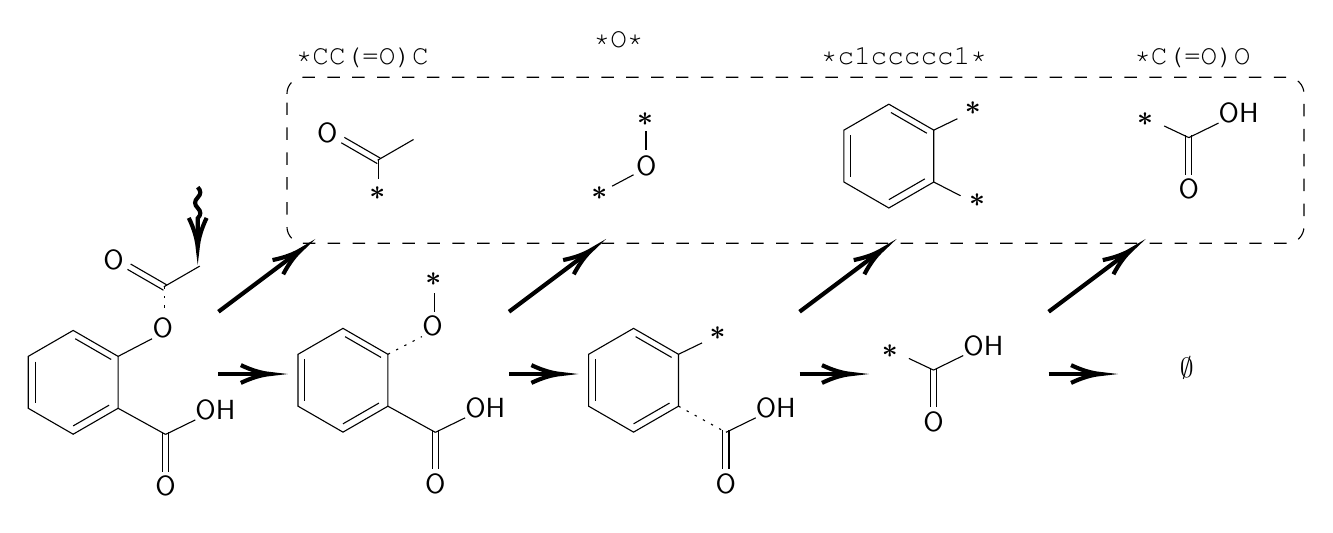
\begin{tikzpicture}[x=0.75pt,y=0.75pt,yscale=-1,xscale=1]
%uncomment if require: \path (0,261); %set diagram left start at 0, and has height of 261

%Shape: Regular Polygon [id:dp5441528921455343]
\draw   (40,219) -- (18.35,206.5) -- (18.35,181.5) -- (40,169) -- (61.65,181.5) -- (61.65,206.5) -- cycle ;
%Straight Lines [id:da8353669023127415]
\draw [color={rgb, 255:red, 0; green, 0; blue, 0 }  ,draw opacity=1 ] [dash pattern={on 0.84pt off 2.51pt}]  (84,148) -- (84,161) ;
%Straight Lines [id:da7264741738633573]
\draw    (61.65,206.5) -- (84.52,219.11) ;
%Straight Lines [id:da9419897329918221]
\draw    (83,218) -- (83,237) ;
%Straight Lines [id:da08030707542558835]
\draw    (86,218) -- (86,237) ;
%Straight Lines [id:da5530700734644509]
\draw    (66.18,139.6) -- (83.5,149.6) ;
%Straight Lines [id:da790594687957088]
\draw    (67.68,137) -- (85,147) ;
%Straight Lines [id:da9254167439072243]
\draw    (101,138) -- (83.68,148) ;
%Straight Lines [id:da8637172136187801]
\draw    (98.84,212.11) -- (84.52,219.11) ;
%Shape: Boxed Line [id:dp15467998486140555]
\draw    (58.32,183) -- (41,173) ;
%Shape: Boxed Line [id:dp7874277710723612]
\draw    (21.66,184) -- (21.66,204) ;
%Shape: Boxed Line [id:dp7393760826446616]
\draw    (57.32,205) -- (40,215) ;
%Straight Lines [id:da6253733493164098]
\draw    (61.65,181.5) -- (78,173) ;
%Straight Lines [id:da14339200969487864]
\draw    (187,87) -- (187,96) ;
%Straight Lines [id:da44923721765501834]
\draw    (169.18,78.6) -- (186.5,88.6) ;
%Straight Lines [id:da7396190068173174]
\draw    (170.68,76) -- (188,86) ;
%Straight Lines [id:da2642417615054462]
\draw    (204,77) -- (186.68,87) ;
%Shape: Regular Polygon [id:dp7544269598266076]
\draw   (170,218) -- (148.35,205.5) -- (148.35,180.5) -- (170,168) -- (191.65,180.5) -- (191.65,205.5) -- cycle ;
%Straight Lines [id:da39600377387545027]
\draw    (214,151) -- (214,160) ;
%Straight Lines [id:da34587108939367583]
\draw    (191.65,205.5) -- (214.52,218.11) ;
%Straight Lines [id:da16212666985437285]
\draw    (213,217) -- (213,236) ;
%Straight Lines [id:da27990188760620915]
\draw    (216,217) -- (216,236) ;
%Straight Lines [id:da12782422389072567]
\draw    (228.84,211.11) -- (214.52,218.11) ;
%Shape: Boxed Line [id:dp12710407729792883]
\draw    (188.32,182) -- (171,172) ;
%Shape: Boxed Line [id:dp06901241168496686]
\draw    (151.66,183) -- (151.66,203) ;
%Shape: Boxed Line [id:dp24332035305461464]
\draw    (187.32,204) -- (170,214) ;
%Straight Lines [id:da4254972054869146]
\draw [color={rgb, 255:red, 0; green, 0; blue, 0 }  ,draw opacity=1 ] [dash pattern={on 0.84pt off 2.51pt}]  (191.65,180.5) -- (208,172) ;
%Straight Lines [id:da35759409213918647]
\draw    (316,73) -- (316,82) ;
%Straight Lines [id:da5439851805644256]
\draw    (299.65,99.5) -- (310,94) ;
%Shape: Regular Polygon [id:dp5780688789268227]
\draw   (310,218) -- (288.35,205.5) -- (288.35,180.5) -- (310,168) -- (331.65,180.5) -- (331.65,205.5) -- cycle ;
%Straight Lines [id:da7189531753769425]
\draw [color={rgb, 255:red, 0; green, 0; blue, 0 }  ,draw opacity=1 ] [dash pattern={on 0.84pt off 2.51pt}]  (331.65,205.5) -- (354.52,218.11) ;
%Straight Lines [id:da015729760849670926]
\draw    (353,217) -- (353,236) ;
%Straight Lines [id:da508744745614957]
\draw    (356,217) -- (356,236) ;
%Straight Lines [id:da7333901214969005]
\draw    (368.84,211.11) -- (354.52,218.11) ;
%Shape: Boxed Line [id:dp7821116031259598]
\draw    (328.32,182) -- (311,172) ;
%Shape: Boxed Line [id:dp2991980751528647]
\draw    (291.66,183) -- (291.66,203) ;
%Shape: Boxed Line [id:dp23007592478514582]
\draw    (327.32,204) -- (310,214) ;
%Straight Lines [id:da7839141780584493]
\draw    (331.65,180.5) -- (343,175) ;
%Shape: Regular Polygon [id:dp06504553344048047]
\draw   (433,110) -- (411.35,97.5) -- (411.35,72.5) -- (433,60) -- (454.65,72.5) -- (454.65,97.5) -- cycle ;
%Straight Lines [id:da5415663535410995]
\draw    (454.65,97.5) -- (467.52,104.11) ;
%Shape: Boxed Line [id:dp6678344578633082]
\draw    (451.32,74) -- (434,64) ;
%Shape: Boxed Line [id:dp8151982232927417]
\draw    (414.66,75) -- (414.66,95) ;
%Shape: Boxed Line [id:dp7238017036812237]
\draw    (450.32,96) -- (433,106) ;
%Straight Lines [id:da9324796829842863]
\draw    (454.65,72.5) -- (466,67) ;
%Straight Lines [id:da5149286578798244]
\draw    (442.65,182.5) -- (454.52,188.11) ;
%Straight Lines [id:da19919766764775115]
\draw    (453,187) -- (453,206) ;
%Straight Lines [id:da3191045376521391]
\draw    (456,187) -- (456,206) ;
%Straight Lines [id:da7608894861911997]
\draw    (468.84,181.11) -- (454.52,188.11) ;
%Straight Lines [id:da2833824315266147]
\draw    (565.65,70.5) -- (577.52,76.11) ;
%Straight Lines [id:da021587565605220016]
\draw    (576,75) -- (576,94) ;
%Straight Lines [id:da764675922133226]
\draw    (579,75) -- (579,94) ;
%Straight Lines [id:da4168629259527994]
\draw    (591.84,69.11) -- (577.52,76.11) ;
%Shape: Rectangle [id:dp8768800468171065]
\draw  [dash pattern={on 4.5pt off 4.5pt}] (143,55) .. controls (143,50.58) and (146.58,47) .. (151,47) -- (625,47) .. controls (629.42,47) and (633,50.58) .. (633,55) -- (633,119) .. controls (633,123.42) and (629.42,127) .. (625,127) -- (151,127) .. controls (146.58,127) and (143,123.42) .. (143,119) -- cycle ;
%Straight Lines [id:da2386684232536831]
\draw [line width=1.5]    (110,160) -- (147.6,131.8) ;
\draw [shift={(150,130)}, rotate = 503.13] [color={rgb, 255:red, 0; green, 0; blue, 0 }  ][line width=1.5]    (14.21,-4.28) .. controls (9.04,-1.82) and (4.3,-0.39) .. (0,0) .. controls (4.3,0.39) and (9.04,1.82) .. (14.21,4.28)   ;
%Straight Lines [id:da654107192310643]
\draw [line width=1.5]    (110,190) -- (132,190) ;
\draw [shift={(135,190)}, rotate = 180] [color={rgb, 255:red, 0; green, 0; blue, 0 }  ][line width=1.5]    (14.21,-4.28) .. controls (9.04,-1.82) and (4.3,-0.39) .. (0,0) .. controls (4.3,0.39) and (9.04,1.82) .. (14.21,4.28)   ;
%Straight Lines [id:da7007314823593822]
\draw [line width=1.5]    (250,160) -- (287.6,131.8) ;
\draw [shift={(290,130)}, rotate = 503.13] [color={rgb, 255:red, 0; green, 0; blue, 0 }  ][line width=1.5]    (14.21,-4.28) .. controls (9.04,-1.82) and (4.3,-0.39) .. (0,0) .. controls (4.3,0.39) and (9.04,1.82) .. (14.21,4.28)   ;
%Straight Lines [id:da9466136946677108]
\draw [line width=1.5]    (250,190) -- (272,190) ;
\draw [shift={(275,190)}, rotate = 180] [color={rgb, 255:red, 0; green, 0; blue, 0 }  ][line width=1.5]    (14.21,-4.28) .. controls (9.04,-1.82) and (4.3,-0.39) .. (0,0) .. controls (4.3,0.39) and (9.04,1.82) .. (14.21,4.28)   ;
%Straight Lines [id:da30124943836314677]
\draw [line width=1.5]    (390,160) -- (427.6,131.8) ;
\draw [shift={(430,130)}, rotate = 503.13] [color={rgb, 255:red, 0; green, 0; blue, 0 }  ][line width=1.5]    (14.21,-4.28) .. controls (9.04,-1.82) and (4.3,-0.39) .. (0,0) .. controls (4.3,0.39) and (9.04,1.82) .. (14.21,4.28)   ;
%Straight Lines [id:da4416094050725605]
\draw [line width=1.5]    (390,190) -- (412,190) ;
\draw [shift={(415,190)}, rotate = 180] [color={rgb, 255:red, 0; green, 0; blue, 0 }  ][line width=1.5]    (14.21,-4.28) .. controls (9.04,-1.82) and (4.3,-0.39) .. (0,0) .. controls (4.3,0.39) and (9.04,1.82) .. (14.21,4.28)   ;
%Straight Lines [id:da7724041476627761]
\draw [line width=1.5]    (510,160) -- (547.6,131.8) ;
\draw [shift={(550,130)}, rotate = 503.13] [color={rgb, 255:red, 0; green, 0; blue, 0 }  ][line width=1.5]    (14.21,-4.28) .. controls (9.04,-1.82) and (4.3,-0.39) .. (0,0) .. controls (4.3,0.39) and (9.04,1.82) .. (14.21,4.28)   ;
%Straight Lines [id:da10439710720480422]
\draw [line width=1.5]    (510,190) -- (532,190) ;
\draw [shift={(535,190)}, rotate = 180] [color={rgb, 255:red, 0; green, 0; blue, 0 }  ][line width=1.5]    (14.21,-4.28) .. controls (9.04,-1.82) and (4.3,-0.39) .. (0,0) .. controls (4.3,0.39) and (9.04,1.82) .. (14.21,4.28)   ;
%Straight Lines [id:da6206515346709651]
\draw [line width=1.5]    (100,100) .. controls (101.67,101.67) and (101.67,103.33) .. (100,105) .. controls (98.33,106.67) and (98.33,108.33) .. (100,110) .. controls (101.67,111.67) and (101.67,113.33) .. (100,115) -- (100,118) -- (100,126) ;
\draw [shift={(100,129)}, rotate = 270] [color={rgb, 255:red, 0; green, 0; blue, 0 }  ][line width=1.5]    (14.21,-4.28) .. controls (9.04,-1.82) and (4.3,-0.39) .. (0,0) .. controls (4.3,0.39) and (9.04,1.82) .. (14.21,4.28)   ;

% Text Node
\draw (59.5,135) node   [align=left] {\begin{minipage}[lt]{8.67pt}\setlength\topsep{0pt}
\begin{center}
$\displaystyle \mathsf{O}$
\end{center}

\end{minipage}};
% Text Node
\draw  [draw opacity=0]  (74.7,162) -- (91.7,162) -- (91.7,174) -- (74.7,174) -- cycle  ;
\draw (83.2,168) node   [align=left] {\begin{minipage}[lt]{8.67pt}\setlength\topsep{0pt}
\begin{center}
$\displaystyle \mathsf{O}$
\end{center}

\end{minipage}};
% Text Node
\draw  [draw opacity=0][fill={rgb, 255:red, 255; green, 255; blue, 255 }  ,fill opacity=1 ]  (76,238) -- (93,238) -- (93,250) -- (76,250) -- cycle  ;
\draw (84.5,244) node   [align=left] {\begin{minipage}[lt]{8.67pt}\setlength\topsep{0pt}
\begin{center}
$\displaystyle \mathsf{O}$
\end{center}

\end{minipage}};
% Text Node
\draw  [draw opacity=0][fill={rgb, 255:red, 255; green, 255; blue, 255 }  ,fill opacity=1 ]  (96.2,198) -- (113.2,198) -- (113.2,210) -- (96.2,210) -- cycle  ;
\draw (104.7,204) node   [align=left] {\begin{minipage}[lt]{8.67pt}\setlength\topsep{0pt}
\begin{center}
$\displaystyle \mathsf{OH}$
\end{center}

\end{minipage}};
% Text Node
\draw (162.5,74) node   [align=left] {\begin{minipage}[lt]{8.67pt}\setlength\topsep{0pt}
\begin{center}
$\displaystyle \mathsf{O}$
\end{center}

\end{minipage}};
% Text Node
\draw (186.5,105) node   [align=left] {\begin{minipage}[lt]{8.67pt}\setlength\topsep{0pt}
\begin{center}
\textbf{*}
\end{center}

\end{minipage}};
% Text Node
\draw  [draw opacity=0]  (204.7,161) -- (221.7,161) -- (221.7,173) -- (204.7,173) -- cycle  ;
\draw (213.2,167) node   [align=left] {\begin{minipage}[lt]{8.67pt}\setlength\topsep{0pt}
\begin{center}
$\displaystyle \mathsf{O}$
\end{center}

\end{minipage}};
% Text Node
\draw  [draw opacity=0][fill={rgb, 255:red, 255; green, 255; blue, 255 }  ,fill opacity=1 ]  (206,237) -- (223,237) -- (223,249) -- (206,249) -- cycle  ;
\draw (214.5,243) node   [align=left] {\begin{minipage}[lt]{8.67pt}\setlength\topsep{0pt}
\begin{center}
$\displaystyle \mathsf{O}$
\end{center}

\end{minipage}};
% Text Node
\draw  [draw opacity=0][fill={rgb, 255:red, 255; green, 255; blue, 255 }  ,fill opacity=1 ]  (226.2,197) -- (243.2,197) -- (243.2,209) -- (226.2,209) -- cycle  ;
\draw (234.7,203) node   [align=left] {\begin{minipage}[lt]{8.67pt}\setlength\topsep{0pt}
\begin{center}
$\displaystyle \mathsf{OH}$
\end{center}

\end{minipage}};
% Text Node
\draw (213.5,146) node   [align=left] {\begin{minipage}[lt]{8.67pt}\setlength\topsep{0pt}
\begin{center}
\textbf{*}
\end{center}

\end{minipage}};
% Text Node
\draw  [draw opacity=0]  (307.7,83.83) -- (324.7,83.83) -- (324.7,95.83) -- (307.7,95.83) -- cycle  ;
\draw (316.2,89.83) node   [align=left] {\begin{minipage}[lt]{8.67pt}\setlength\topsep{0pt}
\begin{center}
$\displaystyle \mathsf{O}$
\end{center}

\end{minipage}};
% Text Node
\draw (315.5,69) node   [align=left] {\begin{minipage}[lt]{8.67pt}\setlength\topsep{0pt}
\begin{center}
\textbf{*}
\end{center}

\end{minipage}};
% Text Node
\draw  [draw opacity=0][fill={rgb, 255:red, 255; green, 255; blue, 255 }  ,fill opacity=1 ]  (346,237) -- (363,237) -- (363,249) -- (346,249) -- cycle  ;
\draw (354.5,243) node   [align=left] {\begin{minipage}[lt]{8.67pt}\setlength\topsep{0pt}
\begin{center}
$\displaystyle \mathsf{O}$
\end{center}

\end{minipage}};
% Text Node
\draw  [draw opacity=0][fill={rgb, 255:red, 255; green, 255; blue, 255 }  ,fill opacity=1 ]  (366.2,197) -- (383.2,197) -- (383.2,209) -- (366.2,209) -- cycle  ;
\draw (374.7,203) node   [align=left] {\begin{minipage}[lt]{8.67pt}\setlength\topsep{0pt}
\begin{center}
$\displaystyle \mathsf{OH}$
\end{center}

\end{minipage}};
% Text Node
\draw (350.5,172) node   [align=left] {\begin{minipage}[lt]{8.67pt}\setlength\topsep{0pt}
\begin{center}
\textbf{*}
\end{center}

\end{minipage}};
% Text Node
\draw (293.5,105) node   [align=left] {\begin{minipage}[lt]{8.67pt}\setlength\topsep{0pt}
\begin{center}
\textbf{*}
\end{center}

\end{minipage}};
% Text Node
\draw (473.5,64) node   [align=left] {\begin{minipage}[lt]{8.67pt}\setlength\topsep{0pt}
\begin{center}
\textbf{*}
\end{center}

\end{minipage}};
% Text Node
\draw  [draw opacity=0][fill={rgb, 255:red, 255; green, 255; blue, 255 }  ,fill opacity=1 ]  (446,207) -- (463,207) -- (463,219) -- (446,219) -- cycle  ;
\draw (454.5,213) node   [align=left] {\begin{minipage}[lt]{8.67pt}\setlength\topsep{0pt}
\begin{center}
$\displaystyle \mathsf{O}$
\end{center}

\end{minipage}};
% Text Node
\draw  [draw opacity=0][fill={rgb, 255:red, 255; green, 255; blue, 255 }  ,fill opacity=1 ]  (466.2,167) -- (483.2,167) -- (483.2,179) -- (466.2,179) -- cycle  ;
\draw (474.7,173) node   [align=left] {\begin{minipage}[lt]{8.67pt}\setlength\topsep{0pt}
\begin{center}
$\displaystyle \mathsf{OH}$
\end{center}

\end{minipage}};
% Text Node
\draw (433.5,181) node   [align=left] {\begin{minipage}[lt]{8.67pt}\setlength\topsep{0pt}
\begin{center}
\textbf{*}
\end{center}

\end{minipage}};
% Text Node
\draw (475.5,108) node   [align=left] {\begin{minipage}[lt]{8.67pt}\setlength\topsep{0pt}
\begin{center}
\textbf{*}
\end{center}

\end{minipage}};
% Text Node
\draw  [draw opacity=0][fill={rgb, 255:red, 255; green, 255; blue, 255 }  ,fill opacity=1 ]  (569,95) -- (586,95) -- (586,107) -- (569,107) -- cycle  ;
\draw (577.5,101) node   [align=left] {\begin{minipage}[lt]{8.67pt}\setlength\topsep{0pt}
\begin{center}
$\displaystyle \mathsf{O}$
\end{center}

\end{minipage}};
% Text Node
\draw  [draw opacity=0][fill={rgb, 255:red, 255; green, 255; blue, 255 }  ,fill opacity=1 ]  (589.2,55) -- (606.2,55) -- (606.2,67) -- (589.2,67) -- cycle  ;
\draw (597.7,61) node   [align=left] {\begin{minipage}[lt]{8.67pt}\setlength\topsep{0pt}
\begin{center}
$\displaystyle \mathsf{OH}$
\end{center}

\end{minipage}};
% Text Node
\draw (556.5,69) node   [align=left] {\begin{minipage}[lt]{8.67pt}\setlength\topsep{0pt}
\begin{center}
\textbf{*}
\end{center}

\end{minipage}};
% Text Node
\draw (572,180.4) node [anchor=north west][inner sep=0.75pt]    {$\emptyset $};
% Text Node
\draw (146,23.4) node [anchor=north west][inner sep=0.75pt]   [align=left] {\begin{minipage}[lt]{45.56pt}\setlength\topsep{0pt}
\begin{center}
{\fontfamily{pcr}\selectfont *CC(=O)C}
\end{center}

\end{minipage}};
% Text Node
\draw (289,23.4) node [anchor=north west][inner sep=0.75pt]   [align=left] {\begin{minipage}[lt]{18.785pt}\setlength\topsep{0pt}
\begin{center}
{\fontfamily{pcr}\selectfont *O*}
\end{center}

\end{minipage}};
% Text Node
\draw (399,23.4) node [anchor=north west][inner sep=0.75pt]   [align=left] {\begin{minipage}[lt]{56.27pt}\setlength\topsep{0pt}
\begin{center}
{\fontfamily{pcr}\selectfont *c1ccccc1*}
\end{center}

\end{minipage}};
% Text Node
\draw (550,23.4) node [anchor=north west][inner sep=0.75pt]   [align=left] {\begin{minipage}[lt]{40.205000000000005pt}\setlength\topsep{0pt}
\begin{center}
{\fontfamily{pcr}\selectfont *C(=O)O}
\end{center}

\end{minipage}};


\end{tikzpicture}}
    \caption{Fragmentation of the aspirin molecule (SMILES string \texttt{CC(=O)OC1=CC=CC=C1C(=O)O}). In the bottom row, the wavy arrow indicates the first atom according to the SMILES ordering, and dashed bonds are broken according to the BRICS rules. At each iteration, the leftmost fragment is stripped out of the molecule until the remainder cannot be broken further. The derived fragment sequence is displayed in the top row, delimited by a dashed box.}
    \label{fig:fragmentation}
\end{figure}
After the fragmentation phase, the set of molecular graphs $\mathcal{G}$ is transformed in a set of fragment sequences $\Data = \{s_{(i)} = (\Graph{f}_{[1]}, \Graph{f}_{[2]}, \ldots, \Graph{f}_{[|s_{(i)}|]}) \mid \PatternGraph{G}{i} \in \mathcal{G}\}_{i=1}^n$. We also add an additional data structure, a \emph{vocabulary} $V$, which holds the one-hot vector of every unique fragment found during the fragmentation process. We indicate with $V(\Graph{f}_{[i]}) \in \Real^{|V|}$ the one-hot vector in the vocabulary corresponding to fragment $\Graph{f}_{[i]}$, and with $|V|$ the size of the vocabulary.

\subsection{Skip-Gram Embedding of Fragments}
In this phase, we transform the one-hot vectors specifying the fragments into continuous vectors enriched with context semantics. In analogy with the work of \citet{bowman2016sentencescontinuousspace}, we view a sequence of fragments as a \quotes{sentence}; therefore, each fragment is a \quotes{word}. Given a sequence $s = (\Graph{f}_{[1]}, \Graph{f}_{[2]}, \ldots, \Graph{f}_{[|s|]})$ of fragments, this objective corresponds to optimizing the following skipgram loss function \citep{mikolov2014skipgram}:
$$\Loss((\Matrix{E}, \Matrix{E}_{\mathrm{out}}), s) = - \sum_{i=1}^{|s|}\sum_{-w \leq j \leq w} \log p_{\Matrix{E}, \Matrix{E}_{\mathrm{out}}}(\Graph{f}_{[i+j]}| \Graph{f}_{[i]}),\ j \neq 0,$$
where $w$ is called context window, $\Graph{f}_{[i]}$ is an input fragment fragment, and $\Graph{f}_{[i+j]}$ are fragments that occur in the context of $\Graph{f}_{[i]}$. We implement $p_{\Matrix{E}, \Matrix{E}_{\mathrm{out}}}$ as the following neural network:
\begin{align*}
    \Elem{f}{i} &= \Matrix{E}\, V(\Graph{f}_{[i]})\\
    \Elem{o}{i} &= \softmax(\Matrix{E}_{\mathrm{out}}\Elem{f}{i}),
\end{align*}
where $\Matrix{E} \in \Real^{d \times |V|}$ is an embedding matrix and $\Matrix{E}_{\mathrm{out}} \in \Real^{d \times |V|}$ is an output matrix. The model is pretrained with negative sampling \citep{mikolov2014skipgram}. After pretraining, the columns of the embedding matrix $\Matrix{E}$ contain $d$-dimensional embeddings of each fragment in the vocabulary. As a result, fragment embeddings are endowed with context semantics: precisely, embeddings that are close in a sequence of fragments are represented by nearby vectors in embedding space.

\subsection{Model}
Here, we describe the proposed model, detailing how it is trained, and how it can be used for inference and molecular generation.

\subsubsection*{Training}
The model architecture is a standard \gls{vae} \gls{s2s} model for graph generation, composed of an encoder $\Encoder(\Vector{z} \given s)$ and an autoregressive graph decoder $\Decoder(s \given \Vector{z})$, where $s = (\Graph{f}_{[1]}, \Graph{f}_{[2]}, \ldots, \Graph{f}_{[|s|]})$ is a generic input fragment sequence. The encoder is a \gls{rnn} that operates at fragment level and computes the following:
\begin{align*}
    \Elem{f}{i} &= \Matrix{E}\, V(\Graph{f}_{[i]})\\
    \Elem{h}{i} &= \Op{GRU}_{\EncParam}\Par{\Elem{h}{i-1}, \Elem{f}{i}},
\end{align*}
where $\Matrix{E}$ is the pretrained embedding matrix, and $\Elem{h}{0} = \Zeros$ as usual. The final hidden state $\Elem{h}{|s|} \in \Real^h$ is used as a representation of the whole fragment sequence. The sequence representation is then mapped to two vectors as follows:
\begin{align*}
    \MeanVec &= \Matrix{W}_{\EncParam_\mu} \Elem{h}{|s|}\\
    \StdVec &= \Matrix{W}_{\EncParam_\sigma} \Elem{h}{|s|},
\end{align*}
$\MeanVec \in \Real^h$ and $\StdVec \in \Real^h$ represent the mean and variance of the encoding distribution, and $\Matrix{W}_{\EncParam_\mu}, \Matrix{W}_{\EncParam_\sigma} \in \Real^h$ are weight matrices. Subsequently, a latent sample from the encoding distribution is drawn with reparameterization as $\Vector{z} = \MeanVec + \boldsymbol{\eps} \StdVec$, with $\boldsymbol{\eps} \in \Real^h \sim \Normal{\Zeros}{\Identity}$, where $\Identity \in \Real^{h \times h}$ is a unit covariance matrix. The encoder is trained to minimize the \gls{kld} between the distribution parameterized by $\MeanVec$ and $\StdVec$ and a standard Gaussian prior:
$$\Loss(\EncParam, s) = \KLD{\Encoder(\Vector{z} \given s)}{\Normal{\Zeros}{\Identity}}.$$
The decoder is initialized with the latent vector, \ie by setting $\Elem{h'}{0} = \Vector{z}$. Specifically, the decoder is a \gls{rnn} that computes the following:
\begin{align*}
    \Elem{f}{i-1} &= \Matrix{E}\, V(\Graph{f}_{[i-1]})\\
    \Elem{h'}{i} &= \Op{GRU}_{\DecParam}(\Elem{h}{i-1}, \Elem{f}{i-1})\\
    \Elem{o'}{i} &= \softmax\Par{\Matrix{V}_{\DecParam}\Elem{h'}{i} + \Vector{b'}_{\DecParam}},
\end{align*}
where $\Elem{f}{0} = \Matrix{e}\,V(\SOS)$, $\Matrix{E}$ is the shared embedding matrix, and $\Matrix{V} \in \Real^{|V| \times h}$, $\Vector{b'}_{\DecParam} \in \Real^{|V|}$ are the parameters of the softmax output layer. The vector $\Elem{o'}{i} \in \Real^{|V|}$ is the output distribution over all possible fragments in the vocabulary. Each output of the network is compared with the ground truth fragment $\Graph{f}_{[i]}$ with the \gls{ce} function as follows:
$$\Loss(\DecParam, s) = \frac{1}{|s| + 1} \sum_{i=1}^{|s|+1} -\log p_{\DecParam}(\Graph{f}_{[i]} \given \Graph{f}_{[<i]}) = \frac{1}{|s| + 1} \sum_{i=1}^{|s|+1} \Fun{CE}\Par{V(\Graph{f}_{[i]}), \Elem{o'}{i}},$$
where $+1$ is added to account for the end of sequence token. The whole model is trained with \gls{mle} to minimize the following objective function:
$$\argmin_{\Param} \frac{1}{n} \sum_{s \in \Data} \Loss(\EncParam, s) + \Loss(\DecParam, s),$$
where $\Param = (\EncParam, \DecParam)$ as usual. The architecture is shown visually in Figure \ref{fig:fragment-model-training}.

\begin{figure}[h!]
    \centering
    \resizebox{.99\textwidth}{!}{

\tikzset{every picture/.style={line width=0.75pt}} %set default line width to 0.75pt

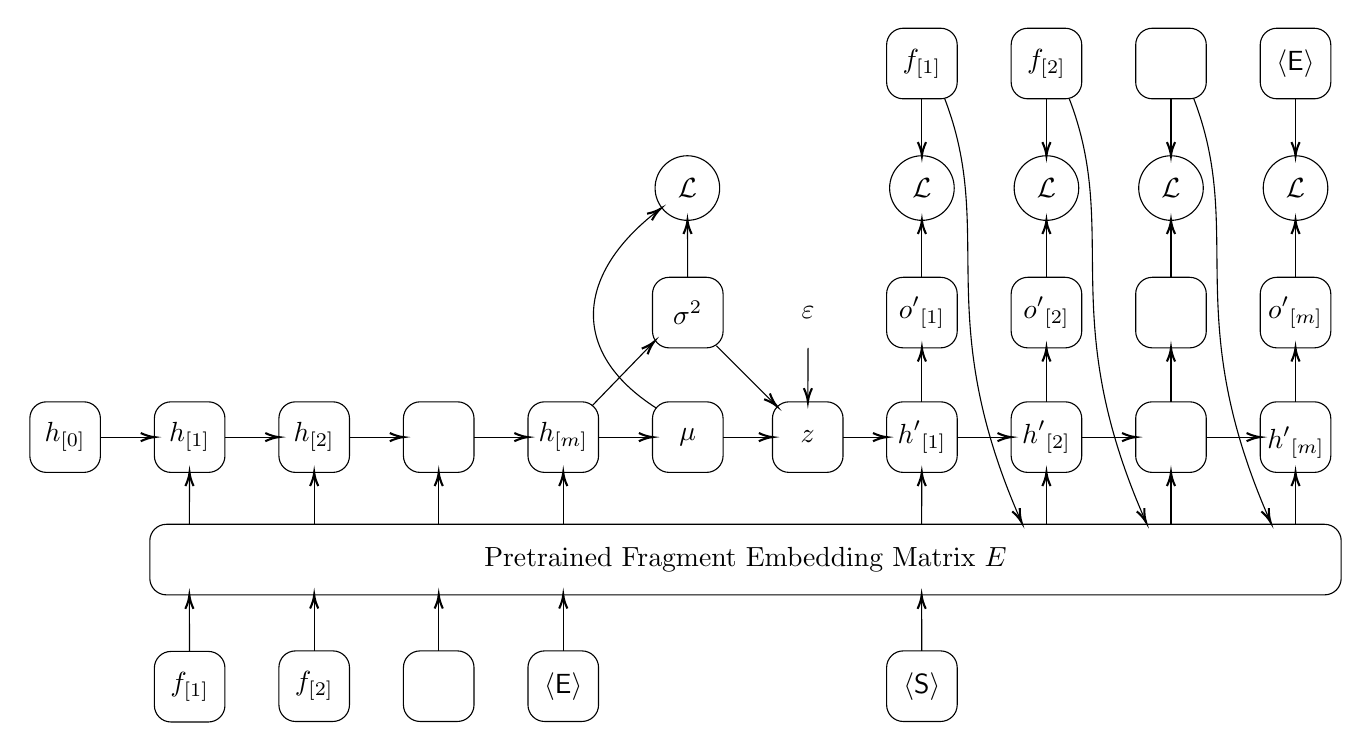
\begin{tikzpicture}[x=0.75pt,y=0.75pt,yscale=-1,xscale=1]
%uncomment if require: \path (0,380); %set diagram left start at 0, and has height of 380

%Curve Lines [id:da9647693741350385]
\draw    (451,62) .. controls (475.78,126.63) and (444.22,166.05) .. (487.34,264.51) ;
\draw [shift={(488,266)}, rotate = 246.11] [color={rgb, 255:red, 0; green, 0; blue, 0 }  ][line width=0.75]    (6.56,-1.97) .. controls (4.17,-0.84) and (1.99,-0.18) .. (0,0) .. controls (1.99,0.18) and (4.17,0.84) .. (6.56,1.97)   ;
%Curve Lines [id:da2808895448373976]
\draw    (511,62) .. controls (535.78,126.63) and (504.22,166.05) .. (547.34,264.51) ;
\draw [shift={(548,266)}, rotate = 246.11] [color={rgb, 255:red, 0; green, 0; blue, 0 }  ][line width=0.75]    (6.56,-1.97) .. controls (4.17,-0.84) and (1.99,-0.18) .. (0,0) .. controls (1.99,0.18) and (4.17,0.84) .. (6.56,1.97)   ;
%Curve Lines [id:da3316276209943081]
\draw    (571,62) .. controls (595.78,126.63) and (564.22,166.05) .. (607.34,264.51) ;
\draw [shift={(608,266)}, rotate = 246.11] [color={rgb, 255:red, 0; green, 0; blue, 0 }  ][line width=0.75]    (6.56,-1.97) .. controls (4.17,-0.84) and (1.99,-0.18) .. (0,0) .. controls (1.99,0.18) and (4.17,0.84) .. (6.56,1.97)   ;
%Straight Lines [id:da7497594724698131]
\draw    (341,181) -- (368.59,208.59) ;
\draw [shift={(370,210)}, rotate = 225] [color={rgb, 255:red, 0; green, 0; blue, 0 }  ][line width=0.75]    (6.56,-1.97) .. controls (4.17,-0.84) and (1.99,-0.18) .. (0,0) .. controls (1.99,0.18) and (4.17,0.84) .. (6.56,1.97)   ;
%Straight Lines [id:da7666415033683152]
\draw    (281,210) -- (309.61,180.44) ;
\draw [shift={(311,179)}, rotate = 494.06] [color={rgb, 255:red, 0; green, 0; blue, 0 }  ][line width=0.75]    (6.56,-1.97) .. controls (4.17,-0.84) and (1.99,-0.18) .. (0,0) .. controls (1.99,0.18) and (4.17,0.84) .. (6.56,1.97)   ;
%Curve Lines [id:da8746649971736793]
\draw    (312,211) .. controls (269.23,183.63) and (273.9,145.77) .. (312.81,115.9) ;
\draw [shift={(314,115)}, rotate = 503.13] [color={rgb, 255:red, 0; green, 0; blue, 0 }  ][line width=0.75]    (6.56,-1.97) .. controls (4.17,-0.84) and (1.99,-0.18) .. (0,0) .. controls (1.99,0.18) and (4.17,0.84) .. (6.56,1.97)   ;

% Text Node
\draw    (70.2,336.25) .. controls (70.2,331.83) and (73.78,328.25) .. (78.2,328.25) -- (96.2,328.25) .. controls (100.62,328.25) and (104.2,331.83) .. (104.2,336.25) -- (104.2,354.25) .. controls (104.2,358.67) and (100.62,362.25) .. (96.2,362.25) -- (78.2,362.25) .. controls (73.78,362.25) and (70.2,358.67) .. (70.2,354.25) -- cycle  ;
\draw (87.2,345.25) node   [align=left] {\begin{minipage}[lt]{20.400000000000002pt}\setlength\topsep{0pt}
\begin{center}
$\displaystyle \Graph{f}_{[ 1]}$
\end{center}

\end{minipage}};
% Text Node
\draw (87,284.16) node   [align=left] {\begin{minipage}[lt]{20.400000000000002pt}\setlength\topsep{0pt}
\begin{center}
\end{center}

\end{minipage}};
% Text Node
\draw (147.2,284) node   [align=left] {\begin{minipage}[lt]{20.400000000000002pt}\setlength\topsep{0pt}
\begin{center}
\end{center}

\end{minipage}};
% Text Node
\draw (207.2,284) node   [align=left] {\begin{minipage}[lt]{20.400000000000002pt}\setlength\topsep{0pt}
\begin{center}
\end{center}

\end{minipage}};
% Text Node
\draw (267.2,284) node   [align=left] {\begin{minipage}[lt]{20.400000000000002pt}\setlength\topsep{0pt}
\begin{center}
\end{center}

\end{minipage}};
% Text Node
\draw    (70.2,216) .. controls (70.2,211.58) and (73.78,208) .. (78.2,208) -- (96.2,208) .. controls (100.62,208) and (104.2,211.58) .. (104.2,216) -- (104.2,234) .. controls (104.2,238.42) and (100.62,242) .. (96.2,242) -- (78.2,242) .. controls (73.78,242) and (70.2,238.42) .. (70.2,234) -- cycle  ;
\draw (87.2,225) node   [align=left] {\begin{minipage}[lt]{20.400000000000002pt}\setlength\topsep{0pt}
\begin{center}
$\displaystyle \boldsymbol{h}_{[ 1]}$
\end{center}

\end{minipage}};
% Text Node
\draw    (130.2,216) .. controls (130.2,211.58) and (133.78,208) .. (138.2,208) -- (156.2,208) .. controls (160.62,208) and (164.2,211.58) .. (164.2,216) -- (164.2,234) .. controls (164.2,238.42) and (160.62,242) .. (156.2,242) -- (138.2,242) .. controls (133.78,242) and (130.2,238.42) .. (130.2,234) -- cycle  ;
\draw (147.2,225) node   [align=left] {\begin{minipage}[lt]{20.400000000000002pt}\setlength\topsep{0pt}
\begin{center}
$\displaystyle \boldsymbol{h}_{[ 2]}$
\end{center}

\end{minipage}};
% Text Node
\draw    (190.2,216) .. controls (190.2,211.58) and (193.78,208) .. (198.2,208) -- (216.2,208) .. controls (220.62,208) and (224.2,211.58) .. (224.2,216) -- (224.2,234) .. controls (224.2,238.42) and (220.62,242) .. (216.2,242) -- (198.2,242) .. controls (193.78,242) and (190.2,238.42) .. (190.2,234) -- cycle  ;
\draw (207.2,225) node   [align=left] {\begin{minipage}[lt]{20.400000000000002pt}\setlength\topsep{0pt}
\begin{center}
$\displaystyle \dotsc $
\end{center}

\end{minipage}};
% Text Node
\draw    (250.2,216) .. controls (250.2,211.58) and (253.78,208) .. (258.2,208) -- (276.2,208) .. controls (280.62,208) and (284.2,211.58) .. (284.2,216) -- (284.2,234) .. controls (284.2,238.42) and (280.62,242) .. (276.2,242) -- (258.2,242) .. controls (253.78,242) and (250.2,238.42) .. (250.2,234) -- cycle  ;
\draw (267.2,225) node   [align=left] {\begin{minipage}[lt]{20.400000000000002pt}\setlength\topsep{0pt}
\begin{center}
$\displaystyle \boldsymbol{h}_{[ m]}$
\end{center}

\end{minipage}};
% Text Node
\draw    (130.2,336) .. controls (130.2,331.58) and (133.78,328) .. (138.2,328) -- (156.2,328) .. controls (160.62,328) and (164.2,331.58) .. (164.2,336) -- (164.2,354) .. controls (164.2,358.42) and (160.62,362) .. (156.2,362) -- (138.2,362) .. controls (133.78,362) and (130.2,358.42) .. (130.2,354) -- cycle  ;
\draw (147.2,345) node   [align=left] {\begin{minipage}[lt]{20.400000000000002pt}\setlength\topsep{0pt}
\begin{center}
$\displaystyle \Graph{f}_{[ 2]}$
\end{center}

\end{minipage}};
% Text Node
\draw    (190.2,336) .. controls (190.2,331.58) and (193.78,328) .. (198.2,328) -- (216.2,328) .. controls (220.62,328) and (224.2,331.58) .. (224.2,336) -- (224.2,354) .. controls (224.2,358.42) and (220.62,362) .. (216.2,362) -- (198.2,362) .. controls (193.78,362) and (190.2,358.42) .. (190.2,354) -- cycle  ;
\draw (207.2,345) node   [align=left] {\begin{minipage}[lt]{20.400000000000002pt}\setlength\topsep{0pt}
\begin{center}
$\displaystyle \dotsc $
\end{center}

\end{minipage}};
% Text Node
\draw    (250.2,336) .. controls (250.2,331.58) and (253.78,328) .. (258.2,328) -- (276.2,328) .. controls (280.62,328) and (284.2,331.58) .. (284.2,336) -- (284.2,354) .. controls (284.2,358.42) and (280.62,362) .. (276.2,362) -- (258.2,362) .. controls (253.78,362) and (250.2,358.42) .. (250.2,354) -- cycle  ;
\draw (267.2,345) node   [align=left] {\begin{minipage}[lt]{20.400000000000002pt}\setlength\topsep{0pt}
\begin{center}
$\displaystyle \langle \mathsf{E} \rangle $
\end{center}

\end{minipage}};
% Text Node
\draw    (423,216) .. controls (423,211.58) and (426.58,208) .. (431,208) -- (449,208) .. controls (453.42,208) and (457,211.58) .. (457,216) -- (457,234) .. controls (457,238.42) and (453.42,242) .. (449,242) -- (431,242) .. controls (426.58,242) and (423,238.42) .. (423,234) -- cycle  ;
\draw (440,225) node   [align=left] {\begin{minipage}[lt]{20.400000000000002pt}\setlength\topsep{0pt}
\begin{center}
$\displaystyle \boldsymbol{h'}_{[ 1]}$
\end{center}

\end{minipage}};
% Text Node
\draw    (483,216) .. controls (483,211.58) and (486.58,208) .. (491,208) -- (509,208) .. controls (513.42,208) and (517,211.58) .. (517,216) -- (517,234) .. controls (517,238.42) and (513.42,242) .. (509,242) -- (491,242) .. controls (486.58,242) and (483,238.42) .. (483,234) -- cycle  ;
\draw (500,225) node   [align=left] {\begin{minipage}[lt]{20.400000000000002pt}\setlength\topsep{0pt}
\begin{center}
$\displaystyle \boldsymbol{h'}_{[ 2]}$
\end{center}

\end{minipage}};
% Text Node
\draw    (543,216) .. controls (543,211.58) and (546.58,208) .. (551,208) -- (569,208) .. controls (573.42,208) and (577,211.58) .. (577,216) -- (577,234) .. controls (577,238.42) and (573.42,242) .. (569,242) -- (551,242) .. controls (546.58,242) and (543,238.42) .. (543,234) -- cycle  ;
\draw (560,225) node   [align=left] {\begin{minipage}[lt]{20.400000000000002pt}\setlength\topsep{0pt}
\begin{center}
$\displaystyle \dotsc $
\end{center}

\end{minipage}};
% Text Node
\draw    (603,216) .. controls (603,211.58) and (606.58,208) .. (611,208) -- (629,208) .. controls (633.42,208) and (637,211.58) .. (637,216) -- (637,234) .. controls (637,238.42) and (633.42,242) .. (629,242) -- (611,242) .. controls (606.58,242) and (603,238.42) .. (603,234) -- cycle  ;
\draw (620,225) node   [align=left] {\begin{minipage}[lt]{20.400000000000002pt}\setlength\topsep{0pt}
\begin{center}
$\displaystyle \boldsymbol{h'}_{[ m]}$
\end{center}

\end{minipage}};
% Text Node
\draw    (423,336) .. controls (423,331.58) and (426.58,328) .. (431,328) -- (449,328) .. controls (453.42,328) and (457,331.58) .. (457,336) -- (457,354) .. controls (457,358.42) and (453.42,362) .. (449,362) -- (431,362) .. controls (426.58,362) and (423,358.42) .. (423,354) -- cycle  ;
\draw (440,345) node   [align=left] {\begin{minipage}[lt]{20.400000000000002pt}\setlength\topsep{0pt}
\begin{center}
$\displaystyle \langle \mathsf{S} \rangle $
\end{center}

\end{minipage}};
% Text Node
\draw (439.8,284.16) node   [align=left] {\begin{minipage}[lt]{20.400000000000002pt}\setlength\topsep{0pt}
\begin{center}
\end{center}

\end{minipage}};
% Text Node
\draw (500,284) node   [align=left] {\begin{minipage}[lt]{20.400000000000002pt}\setlength\topsep{0pt}
\begin{center}
\end{center}

\end{minipage}};
% Text Node
\draw (560,284) node   [align=left] {\begin{minipage}[lt]{20.400000000000002pt}\setlength\topsep{0pt}
\begin{center}
\end{center}

\end{minipage}};
% Text Node
\draw (620,284) node   [align=left] {\begin{minipage}[lt]{20.400000000000002pt}\setlength\topsep{0pt}
\begin{center}
\end{center}

\end{minipage}};
% Text Node
\draw    (423,156) .. controls (423,151.58) and (426.58,148) .. (431,148) -- (449,148) .. controls (453.42,148) and (457,151.58) .. (457,156) -- (457,174) .. controls (457,178.42) and (453.42,182) .. (449,182) -- (431,182) .. controls (426.58,182) and (423,178.42) .. (423,174) -- cycle  ;
\draw (440,165) node   [align=left] {\begin{minipage}[lt]{20.400000000000002pt}\setlength\topsep{0pt}
\begin{center}
$\displaystyle \boldsymbol{o'}_{[ 1]}$
\end{center}

\end{minipage}};
% Text Node
\draw    (483,156) .. controls (483,151.58) and (486.58,148) .. (491,148) -- (509,148) .. controls (513.42,148) and (517,151.58) .. (517,156) -- (517,174) .. controls (517,178.42) and (513.42,182) .. (509,182) -- (491,182) .. controls (486.58,182) and (483,178.42) .. (483,174) -- cycle  ;
\draw (500,165) node   [align=left] {\begin{minipage}[lt]{20.400000000000002pt}\setlength\topsep{0pt}
\begin{center}
$\displaystyle \boldsymbol{o'}_{[ 2]}$
\end{center}

\end{minipage}};
% Text Node
\draw    (543,156) .. controls (543,151.58) and (546.58,148) .. (551,148) -- (569,148) .. controls (573.42,148) and (577,151.58) .. (577,156) -- (577,174) .. controls (577,178.42) and (573.42,182) .. (569,182) -- (551,182) .. controls (546.58,182) and (543,178.42) .. (543,174) -- cycle  ;
\draw (560,165) node   [align=left] {\begin{minipage}[lt]{20.400000000000002pt}\setlength\topsep{0pt}
\begin{center}
$\displaystyle \dotsc $
\end{center}

\end{minipage}};
% Text Node
\draw    (603,156) .. controls (603,151.58) and (606.58,148) .. (611,148) -- (629,148) .. controls (633.42,148) and (637,151.58) .. (637,156) -- (637,174) .. controls (637,178.42) and (633.42,182) .. (629,182) -- (611,182) .. controls (606.58,182) and (603,178.42) .. (603,174) -- cycle  ;
\draw (620,165) node   [align=left] {\begin{minipage}[lt]{20.400000000000002pt}\setlength\topsep{0pt}
\begin{center}
$\displaystyle \boldsymbol{o'}_{[ m]}$
\end{center}

\end{minipage}};
% Text Node
\draw    (440, 105) circle [x radius= 15.56, y radius= 15.56]   ;
\draw (440,105) node   [align=left] {\begin{minipage}[lt]{13.600000000000001pt}\setlength\topsep{0pt}
\begin{center}
$\displaystyle \mathcal{L}$
\end{center}

\end{minipage}};
% Text Node
\draw    (423,36) .. controls (423,31.58) and (426.58,28) .. (431,28) -- (449,28) .. controls (453.42,28) and (457,31.58) .. (457,36) -- (457,54) .. controls (457,58.42) and (453.42,62) .. (449,62) -- (431,62) .. controls (426.58,62) and (423,58.42) .. (423,54) -- cycle  ;
\draw (440,45) node   [align=left] {\begin{minipage}[lt]{20.400000000000002pt}\setlength\topsep{0pt}
\begin{center}
$\displaystyle \Graph{f}_{[ 1]}$
\end{center}

\end{minipage}};
% Text Node
\draw    (483,36) .. controls (483,31.58) and (486.58,28) .. (491,28) -- (509,28) .. controls (513.42,28) and (517,31.58) .. (517,36) -- (517,54) .. controls (517,58.42) and (513.42,62) .. (509,62) -- (491,62) .. controls (486.58,62) and (483,58.42) .. (483,54) -- cycle  ;
\draw (500,45) node   [align=left] {\begin{minipage}[lt]{20.400000000000002pt}\setlength\topsep{0pt}
\begin{center}
$\displaystyle \Graph{f}_{[ 2]}$
\end{center}

\end{minipage}};
% Text Node
\draw    (543,36) .. controls (543,31.58) and (546.58,28) .. (551,28) -- (569,28) .. controls (573.42,28) and (577,31.58) .. (577,36) -- (577,54) .. controls (577,58.42) and (573.42,62) .. (569,62) -- (551,62) .. controls (546.58,62) and (543,58.42) .. (543,54) -- cycle  ;
\draw (560,45) node   [align=left] {\begin{minipage}[lt]{20.400000000000002pt}\setlength\topsep{0pt}
\begin{center}
$\displaystyle \dotsc $
\end{center}

\end{minipage}};
% Text Node
\draw    (603,36) .. controls (603,31.58) and (606.58,28) .. (611,28) -- (629,28) .. controls (633.42,28) and (637,31.58) .. (637,36) -- (637,54) .. controls (637,58.42) and (633.42,62) .. (629,62) -- (611,62) .. controls (606.58,62) and (603,58.42) .. (603,54) -- cycle  ;
\draw (620,45) node   [align=left] {\begin{minipage}[lt]{20.400000000000002pt}\setlength\topsep{0pt}
\begin{center}
$\displaystyle \langle \mathsf{E} \rangle $
\end{center}

\end{minipage}};
% Text Node
\draw    (500, 105) circle [x radius= 15.56, y radius= 15.56]   ;
\draw (500,105) node   [align=left] {\begin{minipage}[lt]{13.600000000000001pt}\setlength\topsep{0pt}
\begin{center}
$\displaystyle \mathcal{L}$
\end{center}

\end{minipage}};
% Text Node
\draw    (560, 105) circle [x radius= 15.56, y radius= 15.56]   ;
\draw (560,105) node   [align=left] {\begin{minipage}[lt]{13.600000000000001pt}\setlength\topsep{0pt}
\begin{center}
$\displaystyle \mathcal{L}$
\end{center}

\end{minipage}};
% Text Node
\draw    (620, 105) circle [x radius= 15.56, y radius= 15.56]   ;
\draw (620,105) node   [align=left] {\begin{minipage}[lt]{13.600000000000001pt}\setlength\topsep{0pt}
\begin{center}
$\displaystyle \mathcal{L}$
\end{center}

\end{minipage}};
% Text Node
\draw    (310.2,216) .. controls (310.2,211.58) and (313.78,208) .. (318.2,208) -- (336.2,208) .. controls (340.62,208) and (344.2,211.58) .. (344.2,216) -- (344.2,234) .. controls (344.2,238.42) and (340.62,242) .. (336.2,242) -- (318.2,242) .. controls (313.78,242) and (310.2,238.42) .. (310.2,234) -- cycle  ;
\draw (327.2,225) node   [align=left] {\begin{minipage}[lt]{20.400000000000002pt}\setlength\topsep{0pt}
\begin{center}
$\displaystyle \boldsymbol{\mu }$
\end{center}

\end{minipage}};
% Text Node
\draw    (310.2,156) .. controls (310.2,151.58) and (313.78,148) .. (318.2,148) -- (336.2,148) .. controls (340.62,148) and (344.2,151.58) .. (344.2,156) -- (344.2,174) .. controls (344.2,178.42) and (340.62,182) .. (336.2,182) -- (318.2,182) .. controls (313.78,182) and (310.2,178.42) .. (310.2,174) -- cycle  ;
\draw (327.2,165) node   [align=left] {\begin{minipage}[lt]{20.400000000000002pt}\setlength\topsep{0pt}
\begin{center}
$\displaystyle \boldsymbol{\sigma }^{2}$
\end{center}

\end{minipage}};
% Text Node
\draw    (327, 105) circle [x radius= 15.56, y radius= 15.56]   ;
\draw (327,105) node   [align=left] {\begin{minipage}[lt]{13.600000000000001pt}\setlength\topsep{0pt}
\begin{center}
$\displaystyle \mathcal{L}$
\end{center}

\end{minipage}};
% Text Node
\draw    (368,216) .. controls (368,211.58) and (371.58,208) .. (376,208) -- (394,208) .. controls (398.42,208) and (402,211.58) .. (402,216) -- (402,234) .. controls (402,238.42) and (398.42,242) .. (394,242) -- (376,242) .. controls (371.58,242) and (368,238.42) .. (368,234) -- cycle  ;
\draw (385,225) node   [align=left] {\begin{minipage}[lt]{20.400000000000002pt}\setlength\topsep{0pt}
\begin{center}
$\displaystyle \boldsymbol{z}$
\end{center}

\end{minipage}};
% Text Node
\draw (385.2,165) node   [align=left] {\begin{minipage}[lt]{20.400000000000002pt}\setlength\topsep{0pt}
\begin{center}
$\displaystyle \boldsymbol{\varepsilon }$
\end{center}

\end{minipage}};
% Text Node
\draw    (68,275) .. controls (68,270.58) and (71.58,267) .. (76,267) -- (634,267) .. controls (638.42,267) and (642,270.58) .. (642,275) -- (642,293) .. controls (642,297.42) and (638.42,301) .. (634,301) -- (76,301) .. controls (71.58,301) and (68,297.42) .. (68,293) -- cycle  ;
\draw (355,284) node   [align=left] {\begin{minipage}[lt]{387.6pt}\setlength\topsep{0pt}
\begin{center}
Pretrained Fragment Embedding Matrix $\displaystyle \boldsymbol{E}$
\end{center}

\end{minipage}};
% Text Node
\draw    (10.2,216) .. controls (10.2,211.58) and (13.78,208) .. (18.2,208) -- (36.2,208) .. controls (40.62,208) and (44.2,211.58) .. (44.2,216) -- (44.2,234) .. controls (44.2,238.42) and (40.62,242) .. (36.2,242) -- (18.2,242) .. controls (13.78,242) and (10.2,238.42) .. (10.2,234) -- cycle  ;
\draw (27.2,225) node   [align=left] {\begin{minipage}[lt]{20.400000000000002pt}\setlength\topsep{0pt}
\begin{center}
$\displaystyle \boldsymbol{h}_{[ 0]}$
\end{center}

\end{minipage}};
% Connection
\draw    (87.14,328.25) -- (87.06,303.16) ;
\draw [shift={(87.06,301.16)}, rotate = 449.81] [color={rgb, 255:red, 0; green, 0; blue, 0 }  ][line width=0.75]    (6.56,-1.97) .. controls (4.17,-0.84) and (1.99,-0.18) .. (0,0) .. controls (1.99,0.18) and (4.17,0.84) .. (6.56,1.97)   ;
% Connection
\draw    (87.06,267.16) -- (87.14,244) ;
\draw [shift={(87.14,242)}, rotate = 450.19] [color={rgb, 255:red, 0; green, 0; blue, 0 }  ][line width=0.75]    (6.56,-1.97) .. controls (4.17,-0.84) and (1.99,-0.18) .. (0,0) .. controls (1.99,0.18) and (4.17,0.84) .. (6.56,1.97)   ;
% Connection
\draw    (147.2,267) -- (147.2,244) ;
\draw [shift={(147.2,242)}, rotate = 450] [color={rgb, 255:red, 0; green, 0; blue, 0 }  ][line width=0.75]    (6.56,-1.97) .. controls (4.17,-0.84) and (1.99,-0.18) .. (0,0) .. controls (1.99,0.18) and (4.17,0.84) .. (6.56,1.97)   ;
% Connection
\draw    (207.2,267) -- (207.2,244) ;
\draw [shift={(207.2,242)}, rotate = 450] [color={rgb, 255:red, 0; green, 0; blue, 0 }  ][line width=0.75]    (6.56,-1.97) .. controls (4.17,-0.84) and (1.99,-0.18) .. (0,0) .. controls (1.99,0.18) and (4.17,0.84) .. (6.56,1.97)   ;
% Connection
\draw    (267.2,267) -- (267.2,244) ;
\draw [shift={(267.2,242)}, rotate = 450] [color={rgb, 255:red, 0; green, 0; blue, 0 }  ][line width=0.75]    (6.56,-1.97) .. controls (4.17,-0.84) and (1.99,-0.18) .. (0,0) .. controls (1.99,0.18) and (4.17,0.84) .. (6.56,1.97)   ;
% Connection
\draw    (104.2,225) -- (128.2,225) ;
\draw [shift={(130.2,225)}, rotate = 180] [color={rgb, 255:red, 0; green, 0; blue, 0 }  ][line width=0.75]    (6.56,-1.97) .. controls (4.17,-0.84) and (1.99,-0.18) .. (0,0) .. controls (1.99,0.18) and (4.17,0.84) .. (6.56,1.97)   ;
% Connection
\draw    (164.2,225) -- (188.2,225) ;
\draw [shift={(190.2,225)}, rotate = 180] [color={rgb, 255:red, 0; green, 0; blue, 0 }  ][line width=0.75]    (6.56,-1.97) .. controls (4.17,-0.84) and (1.99,-0.18) .. (0,0) .. controls (1.99,0.18) and (4.17,0.84) .. (6.56,1.97)   ;
% Connection
\draw    (224.2,225) -- (248.2,225) ;
\draw [shift={(250.2,225)}, rotate = 180] [color={rgb, 255:red, 0; green, 0; blue, 0 }  ][line width=0.75]    (6.56,-1.97) .. controls (4.17,-0.84) and (1.99,-0.18) .. (0,0) .. controls (1.99,0.18) and (4.17,0.84) .. (6.56,1.97)   ;
% Connection
\draw    (147.2,328) -- (147.2,303) ;
\draw [shift={(147.2,301)}, rotate = 450] [color={rgb, 255:red, 0; green, 0; blue, 0 }  ][line width=0.75]    (6.56,-1.97) .. controls (4.17,-0.84) and (1.99,-0.18) .. (0,0) .. controls (1.99,0.18) and (4.17,0.84) .. (6.56,1.97)   ;
% Connection
\draw    (207.2,328) -- (207.2,303) ;
\draw [shift={(207.2,301)}, rotate = 450] [color={rgb, 255:red, 0; green, 0; blue, 0 }  ][line width=0.75]    (6.56,-1.97) .. controls (4.17,-0.84) and (1.99,-0.18) .. (0,0) .. controls (1.99,0.18) and (4.17,0.84) .. (6.56,1.97)   ;
% Connection
\draw    (267.2,328) -- (267.2,303) ;
\draw [shift={(267.2,301)}, rotate = 450] [color={rgb, 255:red, 0; green, 0; blue, 0 }  ][line width=0.75]    (6.56,-1.97) .. controls (4.17,-0.84) and (1.99,-0.18) .. (0,0) .. controls (1.99,0.18) and (4.17,0.84) .. (6.56,1.97)   ;
% Connection
\draw    (457,225) -- (481,225) ;
\draw [shift={(483,225)}, rotate = 180] [color={rgb, 255:red, 0; green, 0; blue, 0 }  ][line width=0.75]    (6.56,-1.97) .. controls (4.17,-0.84) and (1.99,-0.18) .. (0,0) .. controls (1.99,0.18) and (4.17,0.84) .. (6.56,1.97)   ;
% Connection
\draw    (517,225) -- (541,225) ;
\draw [shift={(543,225)}, rotate = 180] [color={rgb, 255:red, 0; green, 0; blue, 0 }  ][line width=0.75]    (6.56,-1.97) .. controls (4.17,-0.84) and (1.99,-0.18) .. (0,0) .. controls (1.99,0.18) and (4.17,0.84) .. (6.56,1.97)   ;
% Connection
\draw    (577,225) -- (601,225) ;
\draw [shift={(603,225)}, rotate = 180] [color={rgb, 255:red, 0; green, 0; blue, 0 }  ][line width=0.75]    (6.56,-1.97) .. controls (4.17,-0.84) and (1.99,-0.18) .. (0,0) .. controls (1.99,0.18) and (4.17,0.84) .. (6.56,1.97)   ;
% Connection
\draw    (439.94,328) -- (439.86,303.16) ;
\draw [shift={(439.86,301.16)}, rotate = 449.81] [color={rgb, 255:red, 0; green, 0; blue, 0 }  ][line width=0.75]    (6.56,-1.97) .. controls (4.17,-0.84) and (1.99,-0.18) .. (0,0) .. controls (1.99,0.18) and (4.17,0.84) .. (6.56,1.97)   ;
% Connection
\draw    (439.86,267.16) -- (439.94,244) ;
\draw [shift={(439.94,242)}, rotate = 450.19] [color={rgb, 255:red, 0; green, 0; blue, 0 }  ][line width=0.75]    (6.56,-1.97) .. controls (4.17,-0.84) and (1.99,-0.18) .. (0,0) .. controls (1.99,0.18) and (4.17,0.84) .. (6.56,1.97)   ;
% Connection
\draw    (500,267) -- (500,244) ;
\draw [shift={(500,242)}, rotate = 450] [color={rgb, 255:red, 0; green, 0; blue, 0 }  ][line width=0.75]    (6.56,-1.97) .. controls (4.17,-0.84) and (1.99,-0.18) .. (0,0) .. controls (1.99,0.18) and (4.17,0.84) .. (6.56,1.97)   ;
% Connection
\draw    (560,267) -- (560,244) ;
\draw [shift={(560,242)}, rotate = 450] [color={rgb, 255:red, 0; green, 0; blue, 0 }  ][line width=0.75]    (6.56,-1.97) .. controls (4.17,-0.84) and (1.99,-0.18) .. (0,0) .. controls (1.99,0.18) and (4.17,0.84) .. (6.56,1.97)   ;
% Connection
\draw    (620,267) -- (620,244) ;
\draw [shift={(620,242)}, rotate = 450] [color={rgb, 255:red, 0; green, 0; blue, 0 }  ][line width=0.75]    (6.56,-1.97) .. controls (4.17,-0.84) and (1.99,-0.18) .. (0,0) .. controls (1.99,0.18) and (4.17,0.84) .. (6.56,1.97)   ;
% Connection
\draw    (440,208) -- (440,184) ;
\draw [shift={(440,182)}, rotate = 450] [color={rgb, 255:red, 0; green, 0; blue, 0 }  ][line width=0.75]    (6.56,-1.97) .. controls (4.17,-0.84) and (1.99,-0.18) .. (0,0) .. controls (1.99,0.18) and (4.17,0.84) .. (6.56,1.97)   ;
% Connection
\draw    (500,208) -- (500,184) ;
\draw [shift={(500,182)}, rotate = 450] [color={rgb, 255:red, 0; green, 0; blue, 0 }  ][line width=0.75]    (6.56,-1.97) .. controls (4.17,-0.84) and (1.99,-0.18) .. (0,0) .. controls (1.99,0.18) and (4.17,0.84) .. (6.56,1.97)   ;
% Connection
\draw    (560,208) -- (560,184) ;
\draw [shift={(560,182)}, rotate = 450] [color={rgb, 255:red, 0; green, 0; blue, 0 }  ][line width=0.75]    (6.56,-1.97) .. controls (4.17,-0.84) and (1.99,-0.18) .. (0,0) .. controls (1.99,0.18) and (4.17,0.84) .. (6.56,1.97)   ;
% Connection
\draw    (620,208) -- (620,184) ;
\draw [shift={(620,182)}, rotate = 450] [color={rgb, 255:red, 0; green, 0; blue, 0 }  ][line width=0.75]    (6.56,-1.97) .. controls (4.17,-0.84) and (1.99,-0.18) .. (0,0) .. controls (1.99,0.18) and (4.17,0.84) .. (6.56,1.97)   ;
% Connection
\draw    (440,62) -- (440,87.44) ;
\draw [shift={(440,89.44)}, rotate = 270] [color={rgb, 255:red, 0; green, 0; blue, 0 }  ][line width=0.75]    (6.56,-1.97) .. controls (4.17,-0.84) and (1.99,-0.18) .. (0,0) .. controls (1.99,0.18) and (4.17,0.84) .. (6.56,1.97)   ;
% Connection
\draw    (440,148) -- (440,122.56) ;
\draw [shift={(440,120.56)}, rotate = 450] [color={rgb, 255:red, 0; green, 0; blue, 0 }  ][line width=0.75]    (6.56,-1.97) .. controls (4.17,-0.84) and (1.99,-0.18) .. (0,0) .. controls (1.99,0.18) and (4.17,0.84) .. (6.56,1.97)   ;
% Connection
\draw    (500,148) -- (500,122.56) ;
\draw [shift={(500,120.56)}, rotate = 450] [color={rgb, 255:red, 0; green, 0; blue, 0 }  ][line width=0.75]    (6.56,-1.97) .. controls (4.17,-0.84) and (1.99,-0.18) .. (0,0) .. controls (1.99,0.18) and (4.17,0.84) .. (6.56,1.97)   ;
% Connection
\draw    (500,62) -- (500,87.44) ;
\draw [shift={(500,89.44)}, rotate = 270] [color={rgb, 255:red, 0; green, 0; blue, 0 }  ][line width=0.75]    (6.56,-1.97) .. controls (4.17,-0.84) and (1.99,-0.18) .. (0,0) .. controls (1.99,0.18) and (4.17,0.84) .. (6.56,1.97)   ;
% Connection
\draw    (560,148) -- (560,122.56) ;
\draw [shift={(560,120.56)}, rotate = 450] [color={rgb, 255:red, 0; green, 0; blue, 0 }  ][line width=0.75]    (6.56,-1.97) .. controls (4.17,-0.84) and (1.99,-0.18) .. (0,0) .. controls (1.99,0.18) and (4.17,0.84) .. (6.56,1.97)   ;
% Connection
\draw    (560,62) -- (560,87.44) ;
\draw [shift={(560,89.44)}, rotate = 270] [color={rgb, 255:red, 0; green, 0; blue, 0 }  ][line width=0.75]    (6.56,-1.97) .. controls (4.17,-0.84) and (1.99,-0.18) .. (0,0) .. controls (1.99,0.18) and (4.17,0.84) .. (6.56,1.97)   ;
% Connection
\draw    (620,148) -- (620,122.56) ;
\draw [shift={(620,120.56)}, rotate = 450] [color={rgb, 255:red, 0; green, 0; blue, 0 }  ][line width=0.75]    (6.56,-1.97) .. controls (4.17,-0.84) and (1.99,-0.18) .. (0,0) .. controls (1.99,0.18) and (4.17,0.84) .. (6.56,1.97)   ;
% Connection
\draw    (620,62) -- (620,87.44) ;
\draw [shift={(620,89.44)}, rotate = 270] [color={rgb, 255:red, 0; green, 0; blue, 0 }  ][line width=0.75]    (6.56,-1.97) .. controls (4.17,-0.84) and (1.99,-0.18) .. (0,0) .. controls (1.99,0.18) and (4.17,0.84) .. (6.56,1.97)   ;
% Connection
\draw    (284.2,225) -- (308.2,225) ;
\draw [shift={(310.2,225)}, rotate = 180] [color={rgb, 255:red, 0; green, 0; blue, 0 }  ][line width=0.75]    (6.56,-1.97) .. controls (4.17,-0.84) and (1.99,-0.18) .. (0,0) .. controls (1.99,0.18) and (4.17,0.84) .. (6.56,1.97)   ;
% Connection
\draw    (327.14,148) -- (327.06,122.56) ;
\draw [shift={(327.05,120.56)}, rotate = 449.81] [color={rgb, 255:red, 0; green, 0; blue, 0 }  ][line width=0.75]    (6.56,-1.97) .. controls (4.17,-0.84) and (1.99,-0.18) .. (0,0) .. controls (1.99,0.18) and (4.17,0.84) .. (6.56,1.97)   ;
% Connection
\draw    (402,225) -- (421,225) ;
\draw [shift={(423,225)}, rotate = 180] [color={rgb, 255:red, 0; green, 0; blue, 0 }  ][line width=0.75]    (6.56,-1.97) .. controls (4.17,-0.84) and (1.99,-0.18) .. (0,0) .. controls (1.99,0.18) and (4.17,0.84) .. (6.56,1.97)   ;
% Connection
\draw    (344.2,225) -- (366,225) ;
\draw [shift={(368,225)}, rotate = 180] [color={rgb, 255:red, 0; green, 0; blue, 0 }  ][line width=0.75]    (6.56,-1.97) .. controls (4.17,-0.84) and (1.99,-0.18) .. (0,0) .. controls (1.99,0.18) and (4.17,0.84) .. (6.56,1.97)   ;
% Connection
\draw    (385.14,182) -- (385.06,206) ;
\draw [shift={(385.06,208)}, rotate = 270.19] [color={rgb, 255:red, 0; green, 0; blue, 0 }  ][line width=0.75]    (6.56,-1.97) .. controls (4.17,-0.84) and (1.99,-0.18) .. (0,0) .. controls (1.99,0.18) and (4.17,0.84) .. (6.56,1.97)   ;
% Connection
\draw    (44.2,225) -- (68.2,225) ;
\draw [shift={(70.2,225)}, rotate = 180] [color={rgb, 255:red, 0; green, 0; blue, 0 }  ][line width=0.75]    (6.56,-1.97) .. controls (4.17,-0.84) and (1.99,-0.18) .. (0,0) .. controls (1.99,0.18) and (4.17,0.84) .. (6.56,1.97)   ;

\end{tikzpicture}}
    \caption{The architecture of the proposed generative model of fragment sequences.}
    \label{fig:fragment-model-training}
\end{figure}

\subsubsection*{Generation}
Generation starts by sampling a latent point $\Vector{z} \in \Real^h$ from the standard gaussian $\Normal{\Zeros}{\Matrix{I}}$,
and setting $\Vector{z} = \Elem{h}{0}$ to initialize the decoder. The initial hidden state is fed to the network together with the starting token $V(\SOS)$. At each step, the network produces a conditional output distribution on every possible word in the vocabulary, from which a fragment $\Graph{\hat{f}}_{[i]}$ is taken using greedy sampling. The sampled token then becomes the input of the next decoding step, together with the updated hidden state. The process is repeated until the end of sequence token $\EOS$ is sampled, at which point the generation is interrupted. The fragments of the sampled sequence $(\Graph{\hat{f}}_{[1]},\Graph{\hat{f}}_{[2]}, \ldots, \EOS)$ are then joined together in the same order to form a novel molecule. Figure \ref{fig:fragment-model-sampling} shows the process visually.
\begin{figure}[h!]
    \centering
    \resizebox{.55\textwidth}{!}{

\tikzset{every picture/.style={line width=0.75pt}} %set default line width to 0.75pt

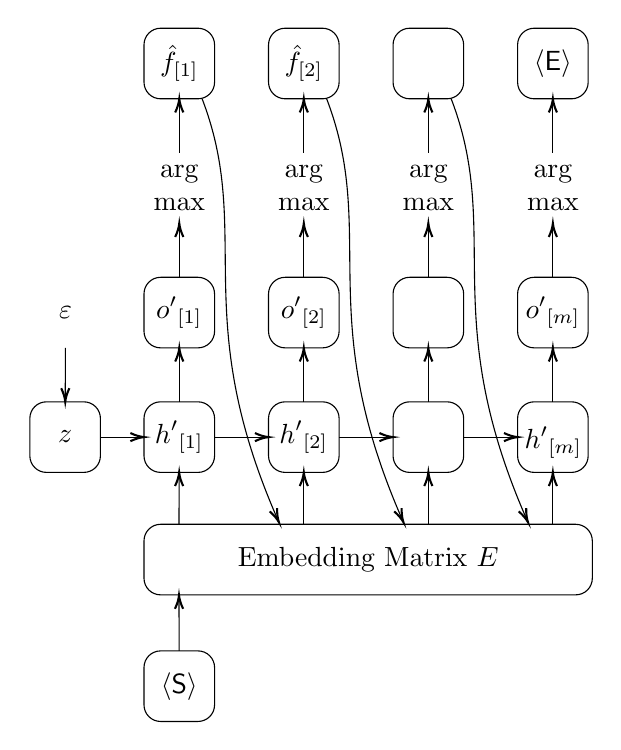
\begin{tikzpicture}[x=0.75pt,y=0.75pt,yscale=-1,xscale=1]
%uncomment if require: \path (0,409); %set diagram left start at 0, and has height of 409

%Curve Lines [id:da9228649105325042]
\draw    (281,47) .. controls (305.78,111.63) and (274.22,151.05) .. (317.34,249.51) ;
\draw [shift={(318,251)}, rotate = 246.11] [color={rgb, 255:red, 0; green, 0; blue, 0 }  ][line width=0.75]    (6.56,-1.97) .. controls (4.17,-0.84) and (1.99,-0.18) .. (0,0) .. controls (1.99,0.18) and (4.17,0.84) .. (6.56,1.97)   ;
%Curve Lines [id:da247291350575354]
\draw    (341,47) .. controls (365.78,111.63) and (334.22,151.05) .. (377.34,249.51) ;
\draw [shift={(378,251)}, rotate = 246.11] [color={rgb, 255:red, 0; green, 0; blue, 0 }  ][line width=0.75]    (6.56,-1.97) .. controls (4.17,-0.84) and (1.99,-0.18) .. (0,0) .. controls (1.99,0.18) and (4.17,0.84) .. (6.56,1.97)   ;
%Curve Lines [id:da2556991067171255]
\draw    (401,47) .. controls (425.78,111.63) and (394.22,151.05) .. (437.34,249.51) ;
\draw [shift={(438,251)}, rotate = 246.11] [color={rgb, 255:red, 0; green, 0; blue, 0 }  ][line width=0.75]    (6.56,-1.97) .. controls (4.17,-0.84) and (1.99,-0.18) .. (0,0) .. controls (1.99,0.18) and (4.17,0.84) .. (6.56,1.97)   ;

% Text Node
\draw    (253,201) .. controls (253,196.58) and (256.58,193) .. (261,193) -- (279,193) .. controls (283.42,193) and (287,196.58) .. (287,201) -- (287,219) .. controls (287,223.42) and (283.42,227) .. (279,227) -- (261,227) .. controls (256.58,227) and (253,223.42) .. (253,219) -- cycle  ;
\draw (270,210) node   [align=left] {\begin{minipage}[lt]{20.400000000000002pt}\setlength\topsep{0pt}
\begin{center}
$\displaystyle \boldsymbol{h'}_{[ 1]}$
\end{center}

\end{minipage}};
% Text Node
\draw    (313,201) .. controls (313,196.58) and (316.58,193) .. (321,193) -- (339,193) .. controls (343.42,193) and (347,196.58) .. (347,201) -- (347,219) .. controls (347,223.42) and (343.42,227) .. (339,227) -- (321,227) .. controls (316.58,227) and (313,223.42) .. (313,219) -- cycle  ;
\draw (330,210) node   [align=left] {\begin{minipage}[lt]{20.400000000000002pt}\setlength\topsep{0pt}
\begin{center}
$\displaystyle \boldsymbol{h'}_{[ 2]}$
\end{center}

\end{minipage}};
% Text Node
\draw    (373,201) .. controls (373,196.58) and (376.58,193) .. (381,193) -- (399,193) .. controls (403.42,193) and (407,196.58) .. (407,201) -- (407,219) .. controls (407,223.42) and (403.42,227) .. (399,227) -- (381,227) .. controls (376.58,227) and (373,223.42) .. (373,219) -- cycle  ;
\draw (390,210) node   [align=left] {\begin{minipage}[lt]{20.400000000000002pt}\setlength\topsep{0pt}
\begin{center}
$\displaystyle \dotsc $
\end{center}

\end{minipage}};
% Text Node
\draw    (433,201) .. controls (433,196.58) and (436.58,193) .. (441,193) -- (459,193) .. controls (463.42,193) and (467,196.58) .. (467,201) -- (467,219) .. controls (467,223.42) and (463.42,227) .. (459,227) -- (441,227) .. controls (436.58,227) and (433,223.42) .. (433,219) -- cycle  ;
\draw (450,210) node   [align=left] {\begin{minipage}[lt]{20.400000000000002pt}\setlength\topsep{0pt}
\begin{center}
$\displaystyle \boldsymbol{h'}_{[ m]}$
\end{center}

\end{minipage}};
% Text Node
\draw    (253,321) .. controls (253,316.58) and (256.58,313) .. (261,313) -- (279,313) .. controls (283.42,313) and (287,316.58) .. (287,321) -- (287,339) .. controls (287,343.42) and (283.42,347) .. (279,347) -- (261,347) .. controls (256.58,347) and (253,343.42) .. (253,339) -- cycle  ;
\draw (270,330) node   [align=left] {\begin{minipage}[lt]{20.400000000000002pt}\setlength\topsep{0pt}
\begin{center}
$\displaystyle \langle \mathsf{S} \rangle $
\end{center}

\end{minipage}};
% Text Node
\draw (269.8,269.16) node   [align=left] {\begin{minipage}[lt]{20.400000000000002pt}\setlength\topsep{0pt}
\begin{center}
\end{center}

\end{minipage}};
% Text Node
\draw (330,269) node   [align=left] {\begin{minipage}[lt]{20.400000000000002pt}\setlength\topsep{0pt}
\begin{center}
\end{center}

\end{minipage}};
% Text Node
\draw (390,269) node   [align=left] {\begin{minipage}[lt]{20.400000000000002pt}\setlength\topsep{0pt}
\begin{center}
\end{center}

\end{minipage}};
% Text Node
\draw (450,269) node   [align=left] {\begin{minipage}[lt]{20.400000000000002pt}\setlength\topsep{0pt}
\begin{center}
\end{center}

\end{minipage}};
% Text Node
\draw    (253,141) .. controls (253,136.58) and (256.58,133) .. (261,133) -- (279,133) .. controls (283.42,133) and (287,136.58) .. (287,141) -- (287,159) .. controls (287,163.42) and (283.42,167) .. (279,167) -- (261,167) .. controls (256.58,167) and (253,163.42) .. (253,159) -- cycle  ;
\draw (270,150) node   [align=left] {\begin{minipage}[lt]{20.400000000000002pt}\setlength\topsep{0pt}
\begin{center}
$\displaystyle \boldsymbol{o'}_{[ 1]}$
\end{center}

\end{minipage}};
% Text Node
\draw    (313,141) .. controls (313,136.58) and (316.58,133) .. (321,133) -- (339,133) .. controls (343.42,133) and (347,136.58) .. (347,141) -- (347,159) .. controls (347,163.42) and (343.42,167) .. (339,167) -- (321,167) .. controls (316.58,167) and (313,163.42) .. (313,159) -- cycle  ;
\draw (330,150) node   [align=left] {\begin{minipage}[lt]{20.400000000000002pt}\setlength\topsep{0pt}
\begin{center}
$\displaystyle \boldsymbol{o'}_{[ 2]}$
\end{center}

\end{minipage}};
% Text Node
\draw    (373,141) .. controls (373,136.58) and (376.58,133) .. (381,133) -- (399,133) .. controls (403.42,133) and (407,136.58) .. (407,141) -- (407,159) .. controls (407,163.42) and (403.42,167) .. (399,167) -- (381,167) .. controls (376.58,167) and (373,163.42) .. (373,159) -- cycle  ;
\draw (390,150) node   [align=left] {\begin{minipage}[lt]{20.400000000000002pt}\setlength\topsep{0pt}
\begin{center}
$\displaystyle \dotsc $
\end{center}

\end{minipage}};
% Text Node
\draw    (433,141) .. controls (433,136.58) and (436.58,133) .. (441,133) -- (459,133) .. controls (463.42,133) and (467,136.58) .. (467,141) -- (467,159) .. controls (467,163.42) and (463.42,167) .. (459,167) -- (441,167) .. controls (436.58,167) and (433,163.42) .. (433,159) -- cycle  ;
\draw (450,150) node   [align=left] {\begin{minipage}[lt]{20.400000000000002pt}\setlength\topsep{0pt}
\begin{center}
$\displaystyle \boldsymbol{o'}_{[ m]}$
\end{center}

\end{minipage}};
% Text Node
\draw    (253,21) .. controls (253,16.58) and (256.58,13) .. (261,13) -- (279,13) .. controls (283.42,13) and (287,16.58) .. (287,21) -- (287,39) .. controls (287,43.42) and (283.42,47) .. (279,47) -- (261,47) .. controls (256.58,47) and (253,43.42) .. (253,39) -- cycle  ;
\draw (270,30) node   [align=left] {\begin{minipage}[lt]{20.400000000000002pt}\setlength\topsep{0pt}
\begin{center}
$\displaystyle \Graph{\hat{f}}_{[ 1]}$
\end{center}

\end{minipage}};
% Text Node
\draw    (313,21) .. controls (313,16.58) and (316.58,13) .. (321,13) -- (339,13) .. controls (343.42,13) and (347,16.58) .. (347,21) -- (347,39) .. controls (347,43.42) and (343.42,47) .. (339,47) -- (321,47) .. controls (316.58,47) and (313,43.42) .. (313,39) -- cycle  ;
\draw (330,30) node   [align=left] {\begin{minipage}[lt]{20.400000000000002pt}\setlength\topsep{0pt}
\begin{center}
$\displaystyle \Graph{\hat{f}}_{[ 2]}$
\end{center}

\end{minipage}};
% Text Node
\draw    (373,21) .. controls (373,16.58) and (376.58,13) .. (381,13) -- (399,13) .. controls (403.42,13) and (407,16.58) .. (407,21) -- (407,39) .. controls (407,43.42) and (403.42,47) .. (399,47) -- (381,47) .. controls (376.58,47) and (373,43.42) .. (373,39) -- cycle  ;
\draw (390,30) node   [align=left] {\begin{minipage}[lt]{20.400000000000002pt}\setlength\topsep{0pt}
\begin{center}
$\displaystyle \dotsc $
\end{center}

\end{minipage}};
% Text Node
\draw    (433,21) .. controls (433,16.58) and (436.58,13) .. (441,13) -- (459,13) .. controls (463.42,13) and (467,16.58) .. (467,21) -- (467,39) .. controls (467,43.42) and (463.42,47) .. (459,47) -- (441,47) .. controls (436.58,47) and (433,43.42) .. (433,39) -- cycle  ;
\draw (450,30) node   [align=left] {\begin{minipage}[lt]{20.400000000000002pt}\setlength\topsep{0pt}
\begin{center}
$\displaystyle \langle \mathsf{E} \rangle $
\end{center}

\end{minipage}};
% Text Node
\draw    (198,201) .. controls (198,196.58) and (201.58,193) .. (206,193) -- (224,193) .. controls (228.42,193) and (232,196.58) .. (232,201) -- (232,219) .. controls (232,223.42) and (228.42,227) .. (224,227) -- (206,227) .. controls (201.58,227) and (198,223.42) .. (198,219) -- cycle  ;
\draw (215,210) node   [align=left] {\begin{minipage}[lt]{20.400000000000002pt}\setlength\topsep{0pt}
\begin{center}
$\displaystyle \boldsymbol{z}$
\end{center}

\end{minipage}};
% Text Node
\draw (215.2,150) node   [align=left] {\begin{minipage}[lt]{20.400000000000002pt}\setlength\topsep{0pt}
\begin{center}
$\displaystyle \boldsymbol{\varepsilon }$
\end{center}

\end{minipage}};
% Text Node
\draw    (253,260) .. controls (253,255.58) and (256.58,252) .. (261,252) -- (461,252) .. controls (465.42,252) and (469,255.58) .. (469,260) -- (469,278) .. controls (469,282.42) and (465.42,286) .. (461,286) -- (261,286) .. controls (256.58,286) and (253,282.42) .. (253,278) -- cycle  ;
\draw (361,269) node   [align=left] {\begin{minipage}[lt]{144.16pt}\setlength\topsep{0pt}
\begin{center}
Embedding Matrix $\Matrix{E}$
\end{center}

\end{minipage}};
% Text Node
\draw (270,90) node   [align=left] {\begin{minipage}[lt]{20.400000000000002pt}\setlength\topsep{0pt}
\begin{center}
arg\\max
\end{center}

\end{minipage}};
% Text Node
\draw (330,90) node   [align=left] {\begin{minipage}[lt]{20.400000000000002pt}\setlength\topsep{0pt}
\begin{center}
arg\\max
\end{center}

\end{minipage}};
% Text Node
\draw (390,90) node   [align=left] {\begin{minipage}[lt]{20.400000000000002pt}\setlength\topsep{0pt}
\begin{center}
arg\\max
\end{center}

\end{minipage}};
% Text Node
\draw (450,90) node   [align=left] {\begin{minipage}[lt]{20.400000000000002pt}\setlength\topsep{0pt}
\begin{center}
arg\\max
\end{center}

\end{minipage}};
% Connection
\draw    (287,210) -- (311,210) ;
\draw [shift={(313,210)}, rotate = 180] [color={rgb, 255:red, 0; green, 0; blue, 0 }  ][line width=0.75]    (6.56,-1.97) .. controls (4.17,-0.84) and (1.99,-0.18) .. (0,0) .. controls (1.99,0.18) and (4.17,0.84) .. (6.56,1.97)   ;
% Connection
\draw    (347,210) -- (371,210) ;
\draw [shift={(373,210)}, rotate = 180] [color={rgb, 255:red, 0; green, 0; blue, 0 }  ][line width=0.75]    (6.56,-1.97) .. controls (4.17,-0.84) and (1.99,-0.18) .. (0,0) .. controls (1.99,0.18) and (4.17,0.84) .. (6.56,1.97)   ;
% Connection
\draw    (407,210) -- (431,210) ;
\draw [shift={(433,210)}, rotate = 180] [color={rgb, 255:red, 0; green, 0; blue, 0 }  ][line width=0.75]    (6.56,-1.97) .. controls (4.17,-0.84) and (1.99,-0.18) .. (0,0) .. controls (1.99,0.18) and (4.17,0.84) .. (6.56,1.97)   ;
% Connection
\draw    (269.94,313) -- (269.86,288.16) ;
\draw [shift={(269.86,286.16)}, rotate = 449.81] [color={rgb, 255:red, 0; green, 0; blue, 0 }  ][line width=0.75]    (6.56,-1.97) .. controls (4.17,-0.84) and (1.99,-0.18) .. (0,0) .. controls (1.99,0.18) and (4.17,0.84) .. (6.56,1.97)   ;
% Connection
\draw    (269.86,252.16) -- (269.94,229) ;
\draw [shift={(269.94,227)}, rotate = 450.19] [color={rgb, 255:red, 0; green, 0; blue, 0 }  ][line width=0.75]    (6.56,-1.97) .. controls (4.17,-0.84) and (1.99,-0.18) .. (0,0) .. controls (1.99,0.18) and (4.17,0.84) .. (6.56,1.97)   ;
% Connection
\draw    (330,252) -- (330,229) ;
\draw [shift={(330,227)}, rotate = 450] [color={rgb, 255:red, 0; green, 0; blue, 0 }  ][line width=0.75]    (6.56,-1.97) .. controls (4.17,-0.84) and (1.99,-0.18) .. (0,0) .. controls (1.99,0.18) and (4.17,0.84) .. (6.56,1.97)   ;
% Connection
\draw    (390,252) -- (390,229) ;
\draw [shift={(390,227)}, rotate = 450] [color={rgb, 255:red, 0; green, 0; blue, 0 }  ][line width=0.75]    (6.56,-1.97) .. controls (4.17,-0.84) and (1.99,-0.18) .. (0,0) .. controls (1.99,0.18) and (4.17,0.84) .. (6.56,1.97)   ;
% Connection
\draw    (450,252) -- (450,229) ;
\draw [shift={(450,227)}, rotate = 450] [color={rgb, 255:red, 0; green, 0; blue, 0 }  ][line width=0.75]    (6.56,-1.97) .. controls (4.17,-0.84) and (1.99,-0.18) .. (0,0) .. controls (1.99,0.18) and (4.17,0.84) .. (6.56,1.97)   ;
% Connection
\draw    (270,193) -- (270,169) ;
\draw [shift={(270,167)}, rotate = 450] [color={rgb, 255:red, 0; green, 0; blue, 0 }  ][line width=0.75]    (6.56,-1.97) .. controls (4.17,-0.84) and (1.99,-0.18) .. (0,0) .. controls (1.99,0.18) and (4.17,0.84) .. (6.56,1.97)   ;
% Connection
\draw    (330,193) -- (330,169) ;
\draw [shift={(330,167)}, rotate = 450] [color={rgb, 255:red, 0; green, 0; blue, 0 }  ][line width=0.75]    (6.56,-1.97) .. controls (4.17,-0.84) and (1.99,-0.18) .. (0,0) .. controls (1.99,0.18) and (4.17,0.84) .. (6.56,1.97)   ;
% Connection
\draw    (390,193) -- (390,169) ;
\draw [shift={(390,167)}, rotate = 450] [color={rgb, 255:red, 0; green, 0; blue, 0 }  ][line width=0.75]    (6.56,-1.97) .. controls (4.17,-0.84) and (1.99,-0.18) .. (0,0) .. controls (1.99,0.18) and (4.17,0.84) .. (6.56,1.97)   ;
% Connection
\draw    (450,193) -- (450,169) ;
\draw [shift={(450,167)}, rotate = 450] [color={rgb, 255:red, 0; green, 0; blue, 0 }  ][line width=0.75]    (6.56,-1.97) .. controls (4.17,-0.84) and (1.99,-0.18) .. (0,0) .. controls (1.99,0.18) and (4.17,0.84) .. (6.56,1.97)   ;
% Connection
\draw    (232,210) -- (251,210) ;
\draw [shift={(253,210)}, rotate = 180] [color={rgb, 255:red, 0; green, 0; blue, 0 }  ][line width=0.75]    (6.56,-1.97) .. controls (4.17,-0.84) and (1.99,-0.18) .. (0,0) .. controls (1.99,0.18) and (4.17,0.84) .. (6.56,1.97)   ;
% Connection
\draw    (215.14,167) -- (215.06,191) ;
\draw [shift={(215.06,193)}, rotate = 270.19] [color={rgb, 255:red, 0; green, 0; blue, 0 }  ][line width=0.75]    (6.56,-1.97) .. controls (4.17,-0.84) and (1.99,-0.18) .. (0,0) .. controls (1.99,0.18) and (4.17,0.84) .. (6.56,1.97)   ;
% Connection
\draw    (270,73) -- (270,49) ;
\draw [shift={(270,47)}, rotate = 450] [color={rgb, 255:red, 0; green, 0; blue, 0 }  ][line width=0.75]    (6.56,-1.97) .. controls (4.17,-0.84) and (1.99,-0.18) .. (0,0) .. controls (1.99,0.18) and (4.17,0.84) .. (6.56,1.97)   ;
% Connection
\draw    (330,73) -- (330,49) ;
\draw [shift={(330,47)}, rotate = 450] [color={rgb, 255:red, 0; green, 0; blue, 0 }  ][line width=0.75]    (6.56,-1.97) .. controls (4.17,-0.84) and (1.99,-0.18) .. (0,0) .. controls (1.99,0.18) and (4.17,0.84) .. (6.56,1.97)   ;
% Connection
\draw    (390,73) -- (390,49) ;
\draw [shift={(390,47)}, rotate = 450] [color={rgb, 255:red, 0; green, 0; blue, 0 }  ][line width=0.75]    (6.56,-1.97) .. controls (4.17,-0.84) and (1.99,-0.18) .. (0,0) .. controls (1.99,0.18) and (4.17,0.84) .. (6.56,1.97)   ;
% Connection
\draw    (450,73) -- (450,49) ;
\draw [shift={(450,47)}, rotate = 450] [color={rgb, 255:red, 0; green, 0; blue, 0 }  ][line width=0.75]    (6.56,-1.97) .. controls (4.17,-0.84) and (1.99,-0.18) .. (0,0) .. controls (1.99,0.18) and (4.17,0.84) .. (6.56,1.97)   ;
% Connection
\draw    (270,133) -- (270,109) ;
\draw [shift={(270,107)}, rotate = 450] [color={rgb, 255:red, 0; green, 0; blue, 0 }  ][line width=0.75]    (6.56,-1.97) .. controls (4.17,-0.84) and (1.99,-0.18) .. (0,0) .. controls (1.99,0.18) and (4.17,0.84) .. (6.56,1.97)   ;
% Connection
\draw    (330,133) -- (330,109) ;
\draw [shift={(330,107)}, rotate = 450] [color={rgb, 255:red, 0; green, 0; blue, 0 }  ][line width=0.75]    (6.56,-1.97) .. controls (4.17,-0.84) and (1.99,-0.18) .. (0,0) .. controls (1.99,0.18) and (4.17,0.84) .. (6.56,1.97)   ;
% Connection
\draw    (390,133) -- (390,109) ;
\draw [shift={(390,107)}, rotate = 450] [color={rgb, 255:red, 0; green, 0; blue, 0 }  ][line width=0.75]    (6.56,-1.97) .. controls (4.17,-0.84) and (1.99,-0.18) .. (0,0) .. controls (1.99,0.18) and (4.17,0.84) .. (6.56,1.97)   ;
% Connection
\draw    (450,133) -- (450,109) ;
\draw [shift={(450,107)}, rotate = 450] [color={rgb, 255:red, 0; green, 0; blue, 0 }  ][line width=0.75]    (6.56,-1.97) .. controls (4.17,-0.84) and (1.99,-0.18) .. (0,0) .. controls (1.99,0.18) and (4.17,0.84) .. (6.56,1.97)   ;

\end{tikzpicture}}
    \caption{Fragment sequence generation using the proposed model.}
    \label{fig:fragment-model-sampling}
\end{figure}

\subsection{Low-Frequency Masking}
To foster molecule diversity, we start from the observation that the distribution of fragments in the data can be roughly approximated by a power law distribution. In fact, there is usually a small number of fragments with very high frequency, as opposed to a very large number of fragments that occur rarely. Hence, infrequent fragments are unlikely to be sampled during generation. To counter this issue, we develop a strategy which we term Low-Frequency Masking (LFM). During training, we mask fragments with frequency below a certain threshold $k$ with a token composed of its frequency and the number of attachment points. As an example, suppose that fragment \texttt{*Nc1ccc(O*)cc1} occurs 5 times in the dataset, and the threshold is $k=10$. Thus, this fragment is masked with the token \texttt{5\_2}, where 5 denotes its frequency, and 2 denotes the number of attachment points. Similarly, fragment \texttt{*C(=O)N1CCN(Cc2ccccc2)CC1} with frequency of 3 is masked with the token \texttt{3\_1}. In contrast, fragment \texttt{*c1ccccc1OC} with a frequency of 200 is left unmasked, since its frequency is above the threshold. A reverse mapping from the masking tokens to the masked fragments is kept. During sampling, whenever a masking token is sampled, we replace it with a fragment sampled with uniform probability from the corresponding set of masked fragments. This strategy serves a double purpose. Firstly, it greatly reduces vocabulary size during training, speeding up the computations. Secondly, it fosters molecule diversity by indirectly boosting the probability of infrequent fragments, and injecting more randomness in the sampling process at the same time. From another point of view, LFM forces the model to generate molecules mostly composed of very frequent fragments, but with infrequent substructures that may vary uniformly from molecule to molecule.

\section{Experiments}\label{sec:aistats-experiments}
Following, we review our experimental setup, namely how the experiments are conceived, which datasets and evaluation metrics are used, which baselines we compare to, as well as details about the hyper-parameters of our model. In our experiments, we try to provide an empirical answer to the following questions:
\begin{itemize}
    \item Q1: is our fragment-based language model able to increase validity rates?
    \item Q2: is our LFM strategy beneficial to increase uniqueness rates?
\end{itemize}
To answer the first question, we compare our model against character-based baselines, which generate molecules atom by atom. As regards the second question, we perform an ablation study of performances with and without LFM. We also compare against graph-based approaches, to assess performances in relation to models that use more expressive molecule representations.

\subsection{Data}
We experiment on the ZINC dataset \citep{irwin2005zinc}, consisting of $\approx$ 250k drug-like compounds. ZINC is a common benchmark for the generative task; as such, it is used to compare against several baselines. To assess the impact of LFM further, in our ablation study we also test our model variants in the PubChem BioAssay (PCBA) dataset  \citep{gindulyte2016pubchem}, which comprises $\approx$ 440k small molecules. Dataset statistics are presented in Table~\ref{tab:mol-statistics}. We applied some common preprocessing steps before training. In the PCBA dataset, we found 10822 duplicate or invalid molecules, which were removed. During an initial preprocessing phase, we discarded molecules composed of $< 2$ fragments. After the preprocessing, our training samples were $227946$ (ZINC) and $383790$ (PCBA). For completeness, we report that we tried to test our model on the QM9 dataset \citep{ramakrishnan2014qm9} as well, but found out that approximately 70\% of its molecules are composed of a single fragment, making assessment poorly informative due to the small sample size.
\begin{table}[h!]
    \begin{center}
    \caption{Dataset statistics.}\label{tab:mol-statistics}
    \renewcommand{\arraystretch}{1.2}
    \begin{tabular}{lcc}
        \toprule

        \textbf{} & \textbf{ZINC} & \textbf{PCBA}\\
        \midrule
        Total number of molecules     & 249455    & 437929\\
        Molecules with no. fragments $\geq 2$  & 227946 & 383790\\
        Mean number of fragments & 2.24$\pm$0.45 & 2.25$\pm$0.48\\
        Vocabulary size & 168537 & 199835\\
        Vocabulary size (LFM) & 21085 & 35949\\
        Average number of atoms & 23.52$\pm$4.29 & 26.78$\pm$6.76\\
        Average number of bonds & 25.31$\pm$5.07 & 28.98$\pm$7.44\\
        Average number of rings & 2.75$\pm$1.00 & 3.16$\pm$1.05\\
        \bottomrule
    \end{tabular}
    \end{center}
\end{table}

\subsection{Performance Metrics}
Following the standards to evaluate molecular generators, we compare our model with the baselines quantitatively, measuring validity, novelty and uniqueness. Validity is assessed by checking the SMILES of the generated graph through the SMILES validator of the \texttt{rdkit} library in Python \citep{rdkit}. To assess the quality of our samples, we compare the distributions of number of atoms, number of bonds and number of rings between the sampled and generated molecules. Moreover, we compare the distributions of the following molecular properties:
\begin{itemize}
    \item octanol/water Partition coefficient (logP), which measures solubility;
    \item Quantitative Estimate of Drug-likeness \citep{bickerton2012qed} (QED), which measures drug-likeness;
    \item Synthetic Accessibility Score \citep{ertl2009sas} (SAS), which measures ease of synthesis.
\end{itemize}
In both cases, we remove duplicates before the valuation, to ensure unbiasedness.
\subsubsection*{Baselines}
We compare to baselines found in the literature, representing both SMILES and graph-based generative models described in Section \ref{sec:review}. As regards SMILES-based approaches, we consider ChemVAE \citep{gomez2018vaemolecule}, GrammarVAE \citep{kusner2017grammarvae} and SD-VAE \citep{dai2018sdvae}, whereas as regards graph-based models, we compare against GraphVAE \citep{simonovsky2018graphvae}, CGVAE \citep{liu2018cgvae} and NeVAE \citep{samanta2019nevae}.

\subsection{Hyper-Parameters}
We evaluate our model using the same hyper-parameters for both variants, in order to isolate the effect of our contribution from improvements due to hyper-parameter tuning. We set the embedding dimension to 64, the number of recurrent layers to 2, the number of GRU units per layer to 128 and the latent space size to 100. We use the Adam optimizer with an initial learning rate of 0.00001, annealed every epoch by a multiplicative factor of 0.9, a batch size of 128, and a dropout rate of 0.3 applied to the recurrent layers to prevent overfitting. We train the model for 4 epochs: after that, we found empirically that the model started to severely overfit the training set. We use $k=10$ as LFM threshold. The stopping criteria for training is the following: after each epoch, we sample 1000 molecules and measure validity, novelty and uniqueness rates of the sample, stopping whenever the uniqueness rate starts to drop (we found out empirically that samples were stable in terms of validity and novelty rates). After training, we sample 20k molecules for evaluation. We publicly release code and samples for reproducibility\footnote{\url{https://github.com/marcopodda/fragment-based-dgm}}. Baseline results are taken from literature\footnote{We found no results in the literature for the PCBA dataset.}.

\section{Results}
The main results of our experiments are summarized in Table \ref{tab:aistats-results}, and provide the answers to the experimental questions posed in Section \ref{sec:aistats-experiments}. As regards Q1, we observe that our model achieves perfect validity scores in the ZINC dataset, greatly outperforming LM-based models and performing on par with the state of the art. This is true also as regards the PCBA dataset. Since both our variants improve over the LM-based competitors, it is safe to argue that our fragment-based approach can effectively increase validity rates. As regards Q2, we observe an improvement in uniqueness by both our variants, with respect to the LM-based competitors. However, the improvement is noticeably higher whenever the LFM strategy is employed. In the PCBA dataset,this trend is even more apparent. Compared to graph-based models, we see how the model with LFM is now competitive with the state of the art. Lastly, we notice that using LFM yields a small improvement in novelty with respect to the vanilla variant.
\begin{table}[h!]
    \begin{center}
    \caption{Scores obtained by our model against SMILES-based and graph-based baselines. LFM indicates that the model has been trained with Low-Frequency Masking. Performances of our LFM variant are shown in bold.}\label{tab:aistats-results}
    \renewcommand{\arraystretch}{1.2}
    \begin{tabular}{lccccc}
        \toprule
        \textbf{Model} & \textbf{Model Family} & \textbf{Dataset} & \textbf{Valid} & \textbf{Novel} & \textbf{Unique}\\
        \midrule
        ChemVAE     & SMILES    & ZINC & 0.170 & 0.980 & 0.310\\
        GrammarVAE  & SMILES    & ZINC & 0.310 & 1.000 & 0.108\\
        SD-VAE      & SMILES    & ZINC & 0.435 &     - &     -\\
        GraphVAE    & Graph & ZINC & 0.140 & 1.000 & 0.316\\
        CGVAE       & Graph & ZINC & 1.000 & 1.000 & 0.998\\
        NeVAE       & Graph & ZINC & 1.000 & 0.999 & 1.000\\
        \midrule
        Ours        & SMILES    & ZINC & 1.000 & 0.992 & 0.460\\
        \textbf{Ours (LFM)}  & SMILES    & ZINC & \textbf{1.000} & \textbf{0.995} & \textbf{0.998}\\
        \midrule
        Ours        & SMILES    & PCBA & 1.000 & 0.981 & 0.108\\
        \textbf{Ours  (LFM)} & SMILES  & PCBA & \textbf{1.000} & \textbf{0.991} & \textbf{0.972}\\
        \bottomrule
    \end{tabular}
    \end{center}
    \end{table}
In Figure \ref{fig:zinc-props} (for the ZINC dataset) and Figure \ref{fig:pcba-props} (as regards the PCBA dataset), our samples against training compounds are compared, as regards the distribution of the three structural features, and molecular properties listed above. Notice that even without the help of an explicit supervision, generated molecules are qualitatively similar to the training data.
\begin{figure}[h!]
    \centering
    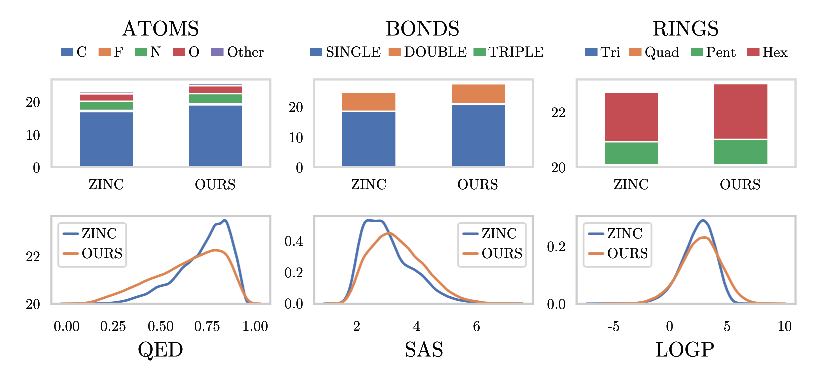
\includegraphics[width=.95\textwidth]{Figures/Chapter7/props-zinc.eps}
    \caption{Comparison of structural and molecular properties between the training and generated samples on the ZINC dataset.}
    \label{fig:zinc-props}
\end{figure}
Finally, Figure \ref{fig:samples} shows two random samples of 30 molecules taken from the ZINC dataset and generated by our model for visual comparison.
\begin{figure}[h!]
    \centering
    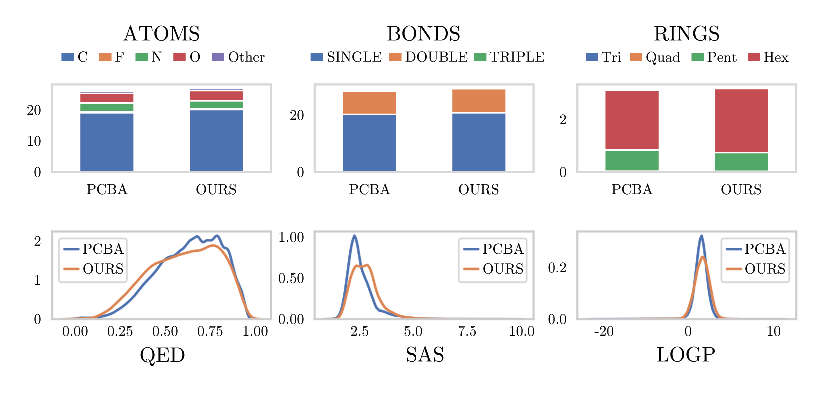
\includegraphics[width=.95\textwidth]{Figures/Chapter7/props-pcba.eps}
    \caption{Comparison of structural and molecular properties between the training and generated samples on the PCBA dataset.}
    \label{fig:pcba-props}
\end{figure}
\begin{figure}[h!]
    \centering
    \begin{subfigure}[b]{0.49\textwidth}
        \centering
        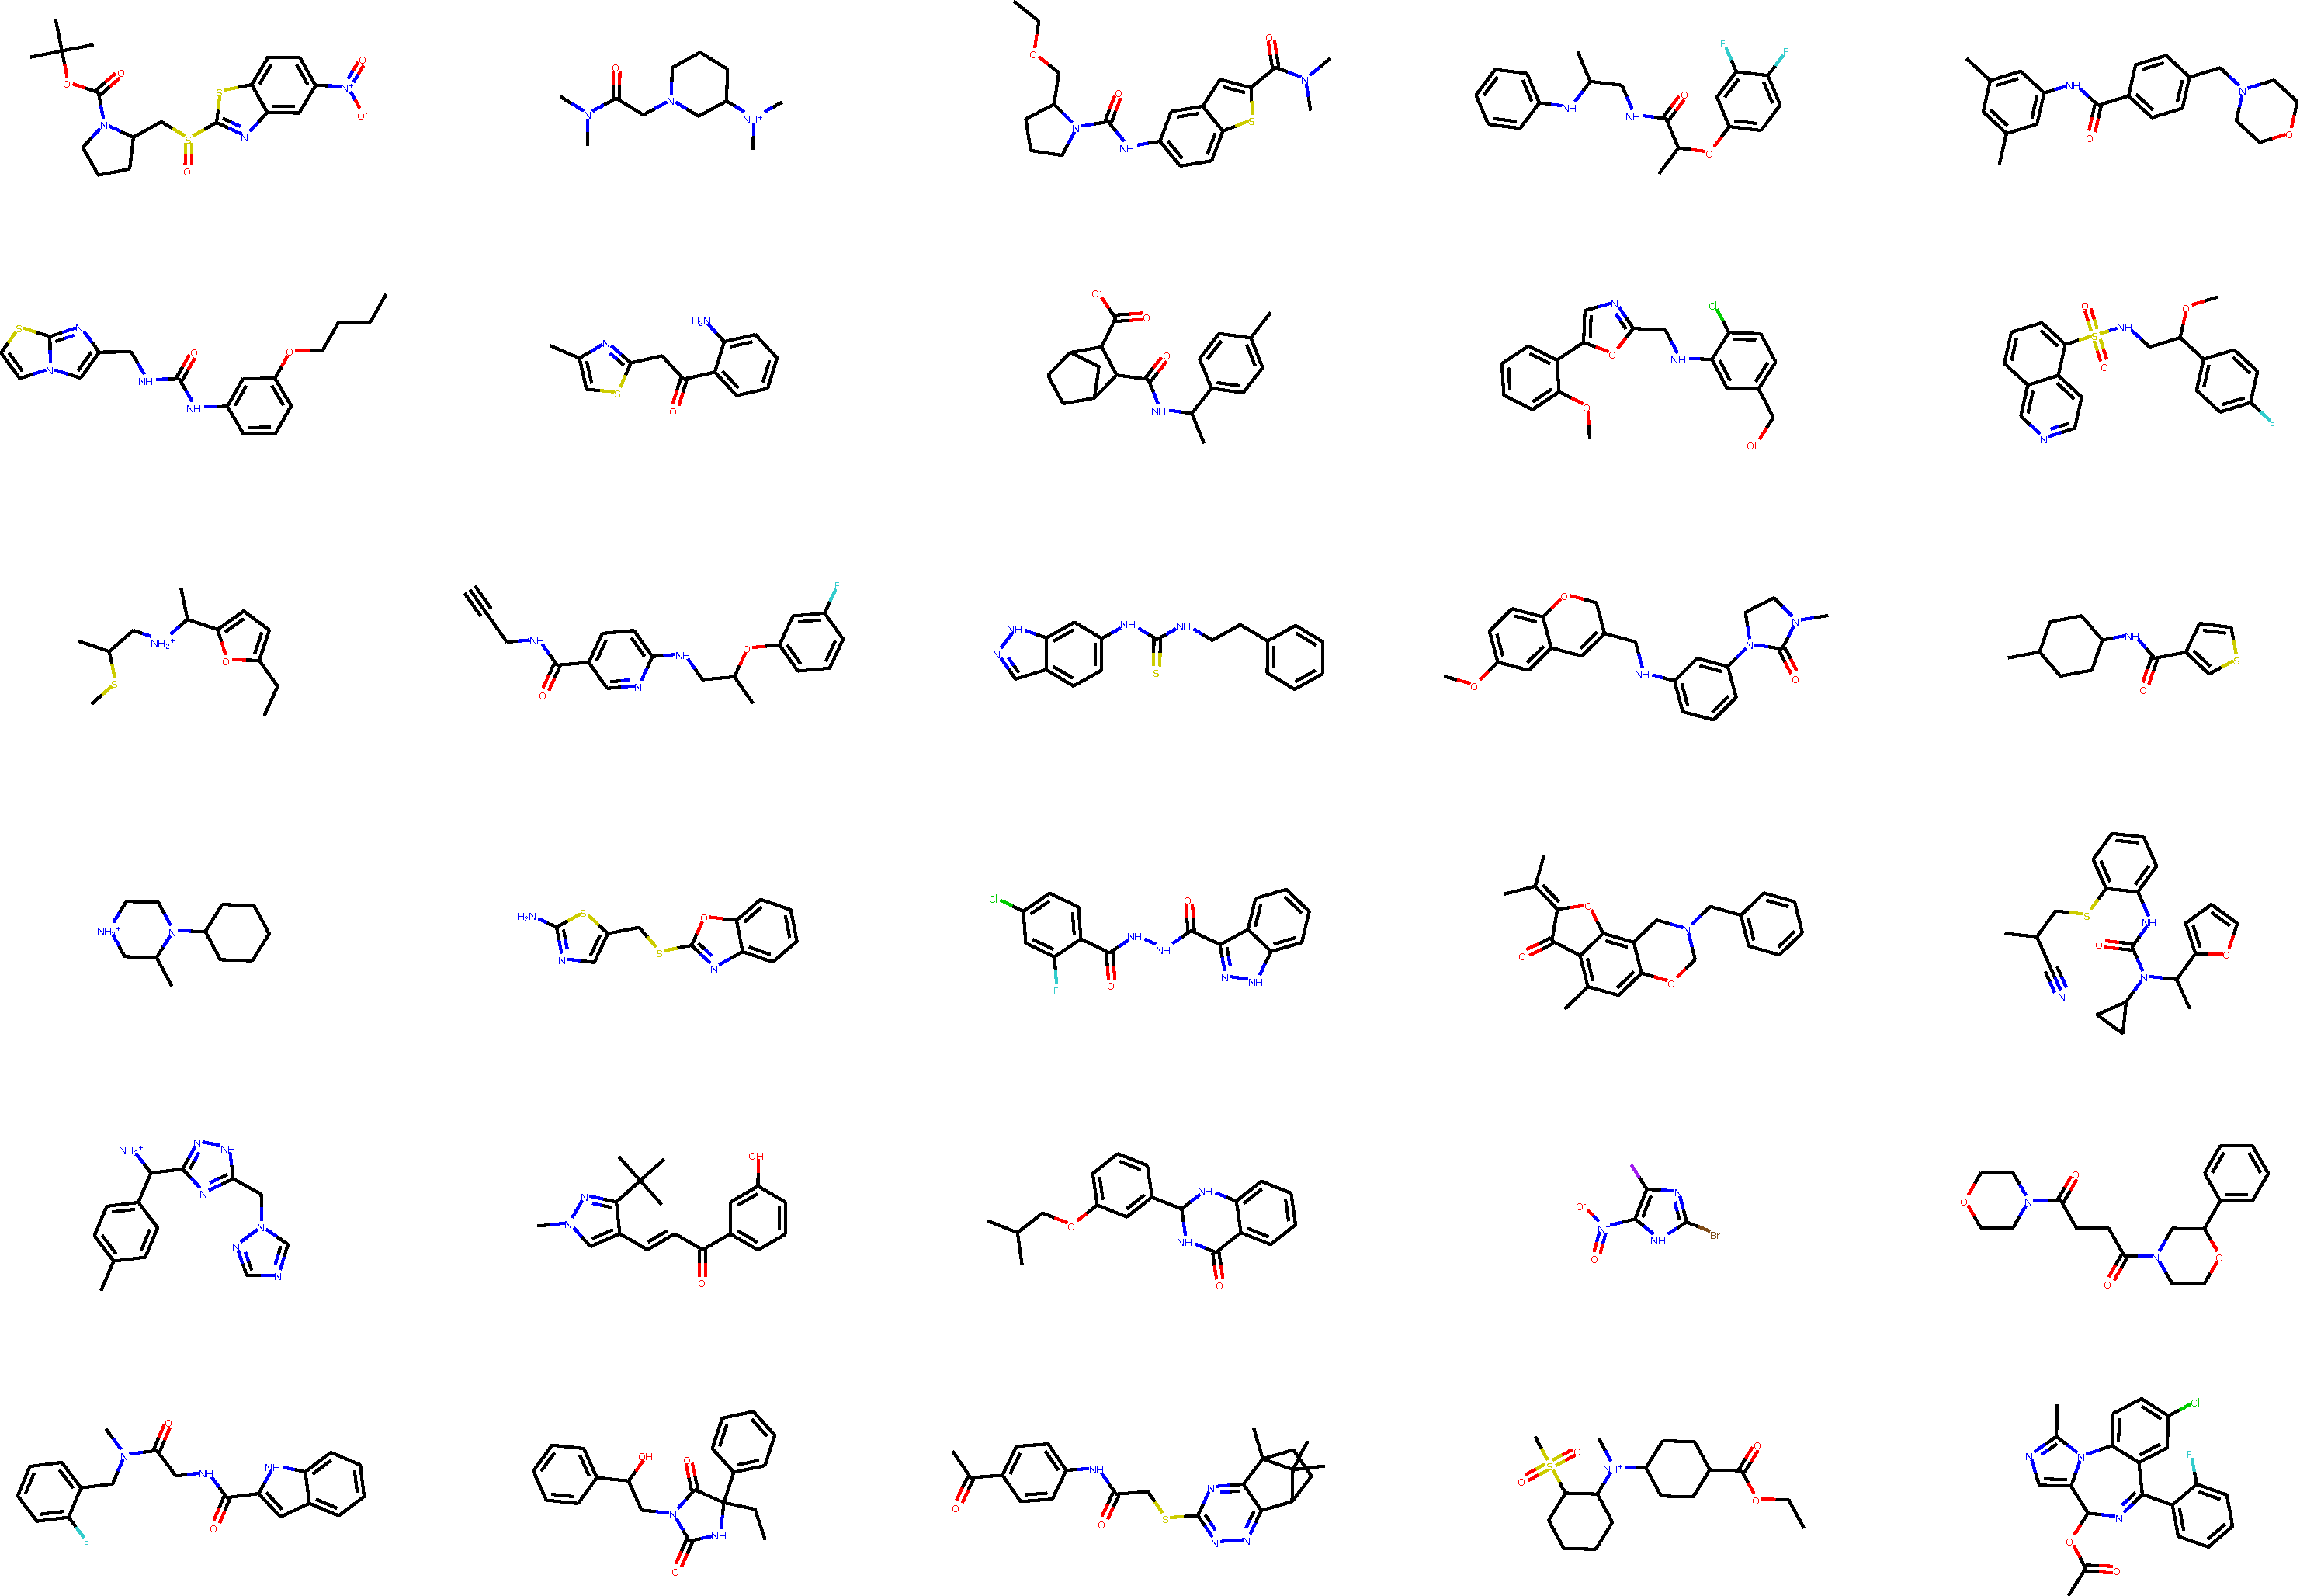
\includegraphics[width=.9\textwidth]{Figures/Chapter7/samples.eps}
        \caption{ZINC}
        \label{fig:zinc-samples}
    \end{subfigure}
    \hfill
    \begin{subfigure}[b]{0.49\textwidth}
        \centering
        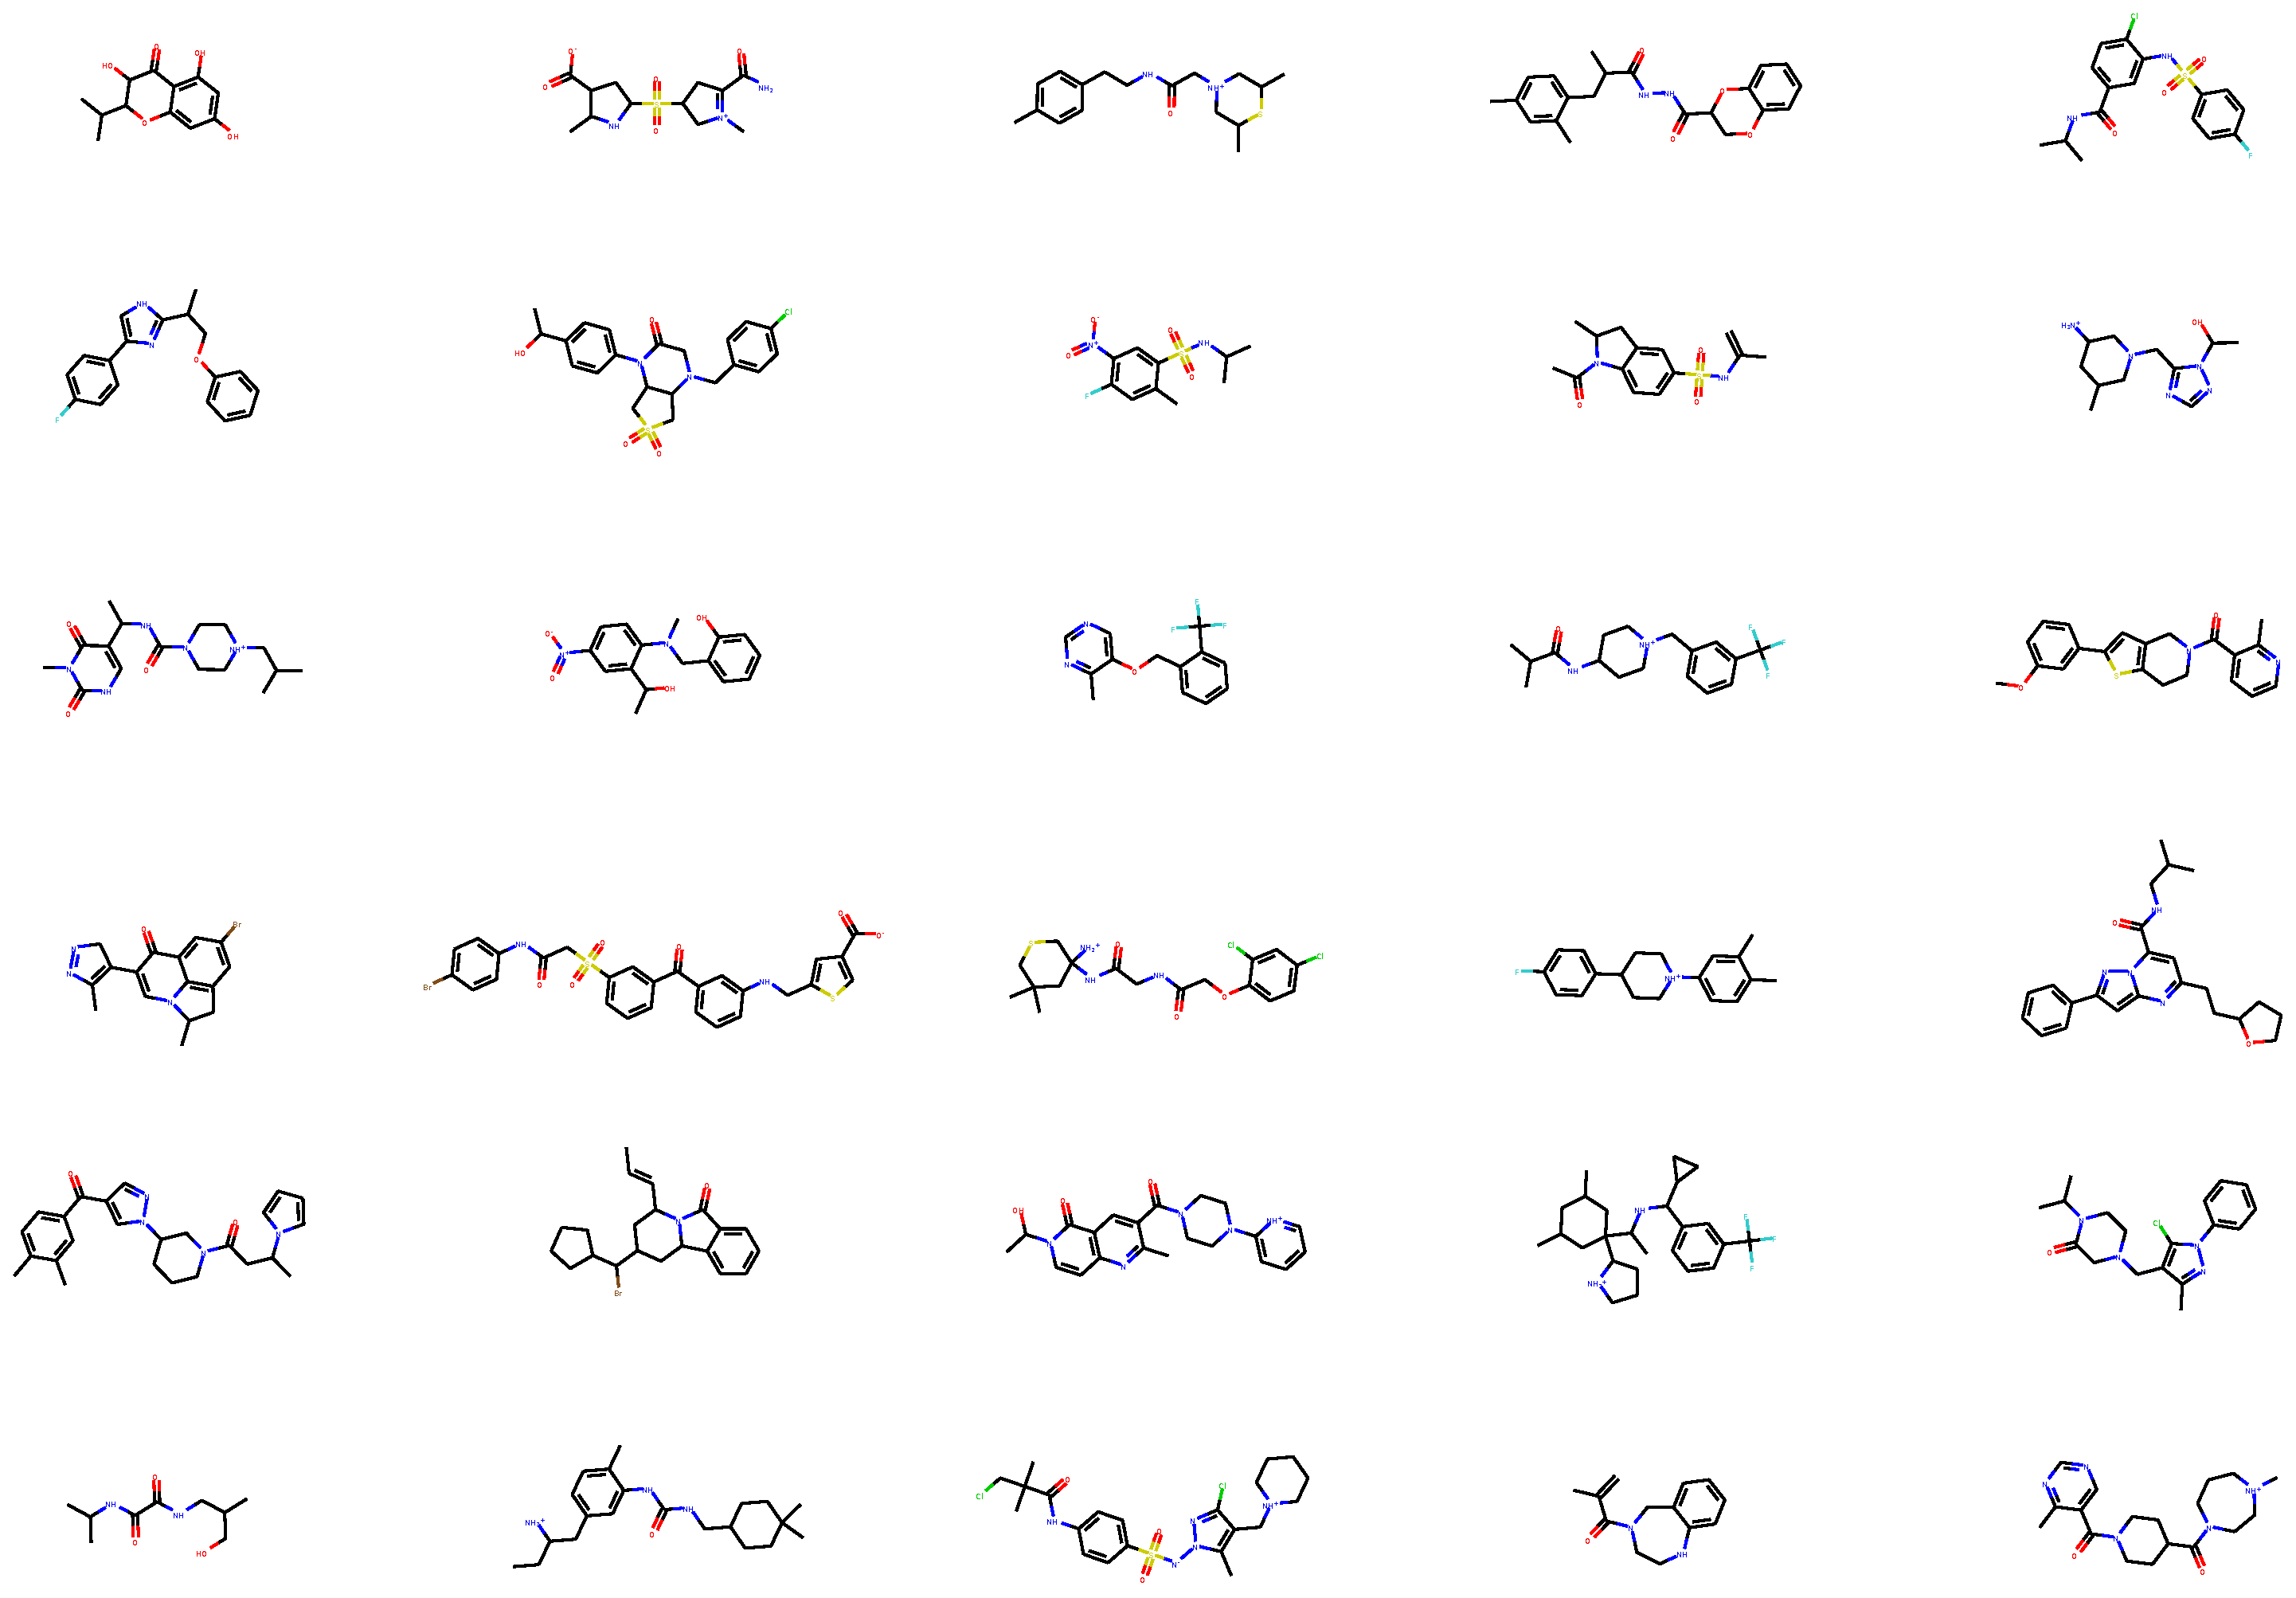
\includegraphics[width=.9\textwidth]{Figures/Chapter7/generated.eps}
        \caption{Generated}
        \label{fig:generated-samples}
    \end{subfigure}
       \caption{A random sample of 30 molecules taken from the ZINC dataset ({\scriptsize A}) and generated by our model ({\scriptsize B}).}
       \label{fig:samples}
\end{figure}